% =====================================================================
% 確定度場の力学 -- 日本語版 (v1.0-ja, 2026-07-20)
% 英語版 dfm-paper.tex v0.9(記録版 = リポジトリタグ paper-v1,
% doi:10.5281/zenodo.21454189)の日本語全訳。国内発表・国内読者向け。
% 学術的な正本(version of record)は英語版であり、本訳と英語版に
% 相違がある場合は英語版が優先する。
% 数値・数式・主張・参考文献は英語版 v0.9 と同一。
% Build: lualatex dfm-paper-ja.tex (2回) — luatexja / HaranoAji フォント
% =====================================================================
\documentclass[a4paper,10pt,twocolumn]{ltjsarticle}

\usepackage{luatexja-fontspec}
\usepackage[haranoaji]{luatexja-preset}
\usepackage{amsmath,amssymb}
\usepackage{bm}
\usepackage{graphicx}
\graphicspath{{figures/}}
\usepackage{booktabs}
\usepackage{array}
\usepackage{xcolor}
\usepackage[unicode,pdfencoding=auto]{hyperref}
\hypersetup{
  colorlinks=true, linkcolor=blue!50!black, citecolor=blue!50!black,
  urlcolor=blue!60!black,
  pdftitle={確定度場の力学:調整可能な慣性系引きずり・逆二乗重力・スピン=熱アナロジーを備えたマッハ的トイ宇宙},
  pdfauthor={今村哲矢 (Tetsuya Imamura)},
  pdfsubject={教育用トイモデル;マッハ的力学;慣性系の引きずり}}

\newcommand{\ud}{\mathrm{d}}
\newcommand{\vect}[1]{\bm{#1}}
\newcommand{\Kt}{K_t}
\newcommand{\Dz}{D_0}

% 図表キャプション体裁
\usepackage{caption}
\captionsetup{font=small,labelfont=bf}

\begin{document}

\twocolumn[{%
\begin{center}
{\LARGE\bfseries 確定度場の力学:調整可能な慣性系引きずり・\\[2pt]
逆二乗重力・スピン=熱アナロジーを備えたマッハ的トイ宇宙\par}
\vspace{6pt}
{\normalsize (Determinacy-Field Mechanics: A Machian Toy Universe with
Tunable Frame Dragging,\\ Inverse-Square Gravity, and Spin-as-Heat
Analogies)\par}
\vspace{12pt}
{\large 今村哲矢(Tetsuya Imamura)\par}
\vspace{2pt}
{\small 独立研究者(Independent Researcher, Tokyo, Japan)\par}
\vspace{4pt}
{\small 2026年7月20日\par}
\vspace{10pt}
\end{center}
\begin{center}
\begin{minipage}{0.92\textwidth}
\small
\textbf{概要} ---
本稿では,教育用トイモデル「確定度場の力学」(Determinacy-Field
Mechanics; DFM)を提示する。このモデルでは,点質量を源として
$w = m/\sqrt{d^2+\varepsilon^2}$ の形で生成される単一のスカラー場 $W$
(「確定度場」)が,局所慣性系を定める重み・重力ポテンシャル・局所的な
時計の進み・光学的屈折率という4つの役割を同時に担い,粒子ごとの符号付き
スピン自由度 $s$ が熱として振る舞う。モデルは2次元ユークリッド背景上の
公理 A1--A13 と更新規則 E1$'$--E11 で完全に規定され,自己完結した単一
HTML ファイルのシミュレータとして実装されており,主要な主張は組み込み
テストスイートによって機械検証されている。1パラメータの背景確定度
$\Dz$ はニュートン的絶対空間($\Dz \to \infty$)と完全に関係論的な
マッハ的空間($\Dz \to 0$)とを連続的に補間し,ニュートンのバケツを
実行可能なパラメータスキャンへと変える。慣性系の引きずりを1のオーダー
まで増幅した場合($k_F = 1$),円盤系は $k_F = 0$ の対照実験に対して
外縁回転速度の緩やかな増強(機械ゲート付き)を示す---これはモデル内部に
おける機構のデモンストレーションである。$k_F = 0$ では力学は厳密に
ニュートン的 $N$ 体重力に帰着する。単一較正 $\Kt = c^2/G$ の下,各
ベンチマークの観測入力を付録に固定した上で,モデルの弱場の時計・光
セクターは GPS 時計オフセット・太陽縁での光の偏向・シャピロ遅延の
主要弱場公式を再現し(公式レベルのベンチマーク一致),重力対光学の比
$1{:}2$ は観測量ごとのフィッティングではなく単一の公理的指数選択
$a = b = 1$ によって固定される。一方,同じ力学は水星の静的第1次
ポストニュートン(1PN)近日点前進を再現せず,この不一致を同一の較正表に
明示する。時計を駆動するのと同じ線素を物質作用に昇格して得られる,
明示的にラベル付けされた測地線オプション(E12)は,追加の自由係数なしに
完全な 1PN 前進($\beta = \gamma = 1$;水星で $+42.98''$/世紀)を回復し,
解析公式に対して機械検証されている(V18--V20)。モデルが主張しないことも
明示する:これは実宇宙の記述ではない;ダークマターの必要性を除去する
ものではない;ローレンツ不変性も因果的伝播も持たない;熱力学セクターは
定量理論ではなくアナロジーである。DFM は,マッハ的着想・弱場現象論・
保存則の帳簿づけを対話的に教え,探究するための,コンパクトで隅々まで
検査可能な実験室として提供される。
\vspace{4pt}

\textbf{訳注} --- 本稿は英語版論文(リポジトリタグ \texttt{paper-v1},
Zenodo \href{https://doi.org/10.5281/zenodo.21454189}%
{doi:10.5281/zenodo.21454189})の著者自身による日本語全訳である。
学術的な正本(version of record)は英語版であり,本訳と英語版に相違が
ある場合は英語版が優先する。数値・数式・主張・参考文献は英語版と同一で
ある。
\end{minipage}
\end{center}
\vspace{14pt}
}]

% =====================================================================
\section{はじめに}
\label{sec:intro}

ニュートンの回転するバケツは,慣性に関する最古の問いの一つを突きつける:
水面は\emph{何に対して}湾曲するのか?~\cite{Newton1687}
ニュートンは「絶対空間」と答えた。マッハはこれに対し,物質の相対的な
配置と運動だけが意味を持ちうる以上,遠方の星々こそが慣性の基準を定める
はずだと反論した~\cite{Mach1883}。のちにシアマは慣性が遠方物質によって
誘導されうる仕組みを素描し~\cite{Sciama1953},バーバーとベルトッティは
関係論的力学に厳密な変分原理による定式化を与えた~\cite{BarbourBertotti1982}。
実宇宙では,一般相対論(GR)がこの問いに微妙な形で決着をつけている:
物質は確かに局所慣性系を引きずる(レンズ=ティリング効果
~\cite{LenseThirring1918})が,その効果は $1/c^2$ の冪で抑制された弱い
ポストニュートン補正であり,地球周回衛星でも年あたりミリ秒角という
微小なものである(Gravity Probe~B と LAGEOS 測距により確認
~\cite{Everitt2011,CiufoliniPavlis2004})。

本稿は意図的に反実仮想的な問いを立て,それに答える最小の動作モデルを
構成する:\emph{もし慣性系の引きずりが1のオーダーの効果だったら,力学は
どのような姿になるか?}
この問いに応えて構成するモデル,確定度場の力学(DFM)は,
\emph{固定ユークリッド背景上のマッハ的トイモデルであって,慣性の基準を
物質分布から創発させるもの}である。
各点質量 $j$ はスカラーの「確定度」
$w_j = m_j/\sqrt{d_j^2+\varepsilon^2}$($\varepsilon \to 0$ で
$\to m_j/d_j$)を寄与し,これはその近傍で空間座標をどれだけ強く
確定させるかを定量化する。
全体場 $W = \Dz + \sum_j w_j$ は,粒子ごとの符号付きスピンスカラー
$s_i$ と併せて,モデル内のあらゆる力学的役割を担う:源の運動の確定度
加重平均が,慣性の拠り所となる局所フレーム $\vect{u}(\vect{r})$ を
定義する;$W$ の勾配が重力加速度である;単一の無次元ポテンシャル
$\psi = W/\Kt$ が局所的な時計の進みと光学的屈折率の双方を定める;
そしてスピンは熱を兼ね,スピン誘起のフレーム回転を通じて圧力を生む。

このモデルは,意図的に,自然の記述の候補ではない。
トイ宇宙の伝統に連なる教育・探究用の道具である:数ページで完全に規定
できるほど小さく(公理 A1--A13,更新規則 E1$'$--E11,帰結 T1--T9),
外部依存のない単一 HTML ファイルのアプリケーションとして動作するほど
具体的で,以下で述べる定量的主張のすべてが実装に埋め込まれた機械検証
テスト(\texttt{HP.verify.all()},14項目,加えて 109 項目の継続的
インテグレーションスイート)で検査されるという点で誠実である。
本稿を通じて「機械検証済み」とは,この組み込み自動スイートにより,
明示されたゲートまたは独立に導出された解析公式に対して検査済みで
あることを意味する---実装の回帰検証であって,独立した実験的検証では
ない。
場とフレームは大域的な配置から瞬時に定まる:DFM には因果的伝播も
ローレンツ不変性もない(第\ref{sec:negative}節)。
主張が特定の初期条件やパラメータ範囲でのみ成り立つ場合は,その旨を
明記し,定理ではなく\emph{条件付き数値命題}とラベル付けする。

\subsection{本稿の貢献}
\label{sec:contributions}

本稿の貢献を,意図する適用範囲とともに述べる:

\begin{enumerate}
\item[C1.]{\bf 最小性と実装可能性。}
13の公理と11の更新規則(A1--A13,E1$'$--E11)からなる体系が,検証済み
パラメータ範囲内で無矛盾であり,単一ファイルの数値実装として動作する
ことを示す---実装による存在証明である。

\item[C2.]{\bf ニュートン重力の構造的分解。}
確定度 $w \propto m/d$ の勾配を加速度とする(公理 A3 と A6)ことで
逆二乗則が得られる。$\nabla(m/d) \propto m/d^2$ だからである。
これは無からの重力の導出では\emph{ない}。重力法則を2つの仮定---場の
距離則 $w \propto m/d$ と勾配応答 $\vect{a} = G\nabla W$---へ分解した
ものである。
なお2次元平面上でガウスの法則と整合する場は $1/d$ で減衰するはずで
あり,DFM は意図的に3次元的距離則を平面上に置いている(擬3次元的
理想化,第\ref{sec:axioms}節)。

\item[C3.]{\bf 弱場 GR との構造的対応。}
パラメータ対応 $\Kt = c^2/G$ の下で,モデルの固有時と光偏向の公式は
弱場 GR と同じ構造を持つ(第\ref{sec:corr}節)。
モデルのバージョン 1.7 以降,時計の進みと屈折は単一ポテンシャル
$\psi$ から $N = e^{-a\psi}$,$A = e^{+b\psi}$ を通じて生成され,指数は
公理として一度だけ $a = b = 1$ に固定される;この選択の下で実効レンズ
係数は導出量 $(a+b)/\Kt = 2/\Kt$ となり,観測量ごとに再調整されることは
決してない。
同じポテンシャルの線素から導かれる測地線オプション E12
(第\ref{sec:e12}節)は,この対応を静的 1PN セクター(水星の近日点前進,
$\beta = \gamma = 1$)にまで拡張する。

\item[C4.]{\bf 絶対空間と関係論的空間の連続補間。}
背景確定度 $\Dz$ はニュートン的絶対空間($\Dz \to \infty$)と完全に
関係論的な空間($\Dz \to 0$)を1つのダイヤルでつなぎ,ニュートンの
バケツ論法を実行可能なパラメータスキャンへ変換する。

\item[C5.]{\bf 外縁速度増強の機構デモンストレーション。}
引きずりを $k_F = 1$ に増幅すると,円盤系は同一初期条件から走らせた
$k_F = 0$ のケプラー的対照ランに対して高い外縁回転速度を示す
(機械ゲート付きの時間平均ゲイン $0.055$,ゲート $\ge 0.03$;6000
ステップ時点の外縁帯比 $1.082$)。
これは\emph{モデル内部での外縁速度増強に対する機構の十分性}を示すもの
であり,回転曲線の平坦性の主張ではなく(第\ref{sec:exp2}節),実在の
銀河についての主張でもない(第\ref{sec:negative}節)。

\item[C6.]{\bf スピン=熱からの創発的熱力学的挙動。}
並進運動をスピンへ変換する接触摩擦,スピン拡散,スピン反発が合わさって,
温度平衡化(第0法則アナロジー)と圧力を生む。

\item[C7.]{\bf 厳密な保存則。}
相反性公理 A13 と改訂規則 E5$'$/E6$'$/E10$'$ により,線運動量と全角運動量
(軌道+スピン)は\emph{方程式レベルで}厳密に保存される(T7,
第\ref{sec:dynamics}節でペアごとに証明);検証ランの有限ステップ数値
残差は単精度の丸め床にあり,時間刻みに依存しない
(表\ref{tab:verify})。
反作用の帳簿づけはさらに,角運動量の外向き輸送,スピン・軌道同期,
潮汐移動のアナロジー(定性的なプリセットデモ)をもたらす。

\item[C8.]{\bf 引きずり歳差の導出と限界の画定。}
順行スピンの中心の周りの順行軌道に対し,E6$'$ は近点を\emph{後退}させ
(機械検査 V6),主要スケーリングは
$\Delta\varpi/\text{周回} \propto -k_F S_c R_c^2/\sqrt{GMa}$ である。
符号とスピン奇の $S_cR_c^2$ 依存性(円盤慣性モーメント
$I = \tfrac12 M R^2$ に対して $\propto J/M_c$)は GR の
レンズ=ティリング近点歳差と平行するが,近傍域での動径冪は異なり
(周回あたり $a^{-1/2}$ 対 レンズ=ティリングの $a^{-3/2}$),静的な
第1次ポストニュートン(1PN)近日点前進は基本力学 E1$'$--E11 では
再現されない(第\ref{sec:negative}節);測地線オプション E12 はこれを
回復する(第\ref{sec:e12}節)。
モデルはまた,背景確定度が円盤のフレーム寄与を遮蔽する背景クロス
オーバースケール $r_{\rm bg} \sim M_d/\Dz$ を示す---これは外縁速度増強が
消えるはずの位置の見積もりであって,平坦区間の予言ではない
(第\ref{sec:exp2}節)。
\end{enumerate}

\subsection{本稿が主張しないこと}
\label{sec:nc-summary}

トイモデル論文の信頼性は過大主張の不在にかかっているため,
第\ref{sec:negative}節で全文を述べる否定的主張をここに要約する:
(1)~DFM は実宇宙の記述として提案されるものではない;
(2)~外縁速度増強のデモはダークマターが不要であることを含意しない;
(3)~モデルはローレンツ不変性を持たず,場の因果的(有限速度)伝播も
持たない;
(4)~モデルは2次元であり,3次元の定量的予言は行わない;
(5)~基本力学 E1$'$--E11 は水星の静的 1PN 近日点前進を再現しない
(明示的にラベル付けされた測地線オプション E12 は再現する,
第\ref{sec:e12}節);
(6)~熱力学セクターは単一粒径に限定された定性的アナロジーであり,
定量的な熱力学理論ではない。

\subsection{先行研究との関係}
\label{sec:prior}

DFM は意図的に,いくつかの文献群から着想を得つつ,そのいずれにも完全には
属さない。
シアマの慣性誘導の提案~\cite{Sciama1953}は精神において最も近い祖先で
ある;DFM は場の理論的素描ではなく,明示的で実行可能な離散力学である
点で異なる。
バーバー=ベルトッティの関係論的力学~\cite{BarbourBertotti1982}は変分
原理から導かれる;DFM は現時点で作用原理を欠いており(未解決問題 L1,
第\ref{sec:limits}節),現象論的簡略化として読まれるべきである。
平坦回転曲線の文献---観測~\cite{RubinFord1970},CMB とレンズ統計に
制約されたダークマター解釈~\cite{Planck2018},MOND~\cite{Milgrom1983}---は
ここでは,モデル内部で示す第三の機構クラス(引きずり増幅)の文脈として
のみ関係する。
GR の重力磁気効果だけで平坦回転曲線を説明できるという主張がなされ
~\cite{CooperstockTieu2005,Ludwig2021},源のモデル・特異物質層・
重力磁気寄与の大きさに関する後続解析によって反論されてきた
~\cite{FuchsPhleps2006,Korzynski2007,LasenbyHobsonBarker2023};
DFM はこの論争に加わらない。$k_F$ を自由なダイヤルとして反実仮想を
研究するからである。
古典力学そのものの関係論的再定式化にはバーバー=ベルトッティ以後も
継続する文献がある:リンデン=ベルとカッツは絶対空間なしの力学が
全角運動量ゼロの宇宙におけるニュートン力学と等価であることを示し
~\cite{LyndenBellKatz1995},アシスはマッハ原理のウェーバー力による実装を
展開した~\cite{Assis1999};DFM は動機を共有しつつ,変分的厳密さを
実行可能な場の構成と引き換えにしている。
重力場中の光の光学媒質的定式化は古典的研究に遡る~\cite{deFelice1971};
本稿の光規則 E8R はその直系の子孫であり,加えて媒質がフレーム場によって
\emph{移流}される。
運動する媒質に運ばれる光は音響的・アナログ重力の定義的構造でもある---
アンルーの音響的地平線~\cite{Unruh1981},およびバルセロ・リベラティ・
ヴィッサーの総説するアナログ重力プログラム
~\cite{BarceloLiberatiVisser2005}---E8R はその単純な一員である
(流れ場 $\vect{u}$ を持つ実効的な音響型幾何)。ただし DFM は地平線
熱力学の主張は行わない。
重力と慣性が創発現象かもしれないという姿勢~\cite{Verlinde2017}は共有
するが,熱力学的・ホログラフィック的導出は試みない。
最後に,スピン=熱セクターは粒状気体運動論
~\cite{BrilliantovPoschel2004}の親類であるが,そこには対応物のない
非局所スピン反発を持つ。

\subsection{構成}

第\ref{sec:axioms}節で公理を,第\ref{sec:dynamics}節で更新規則を述べる。
第\ref{sec:corr}節ではニュートン的帰着,標準観測入力からのベンチマーク
較正を伴う弱場 GR 対応(基本力学の水星不一致を含む),構造的相違点,
および静的 1PN セクターを回復する測地線オプション E12 を与える。
第\ref{sec:experiments}節では機械検証済みの結果を伴う6つの数値実験を
提示する。
第\ref{sec:negative}節で限界と否定的主張を述べ,
第\ref{sec:conclusion}節で今後の課題を概観する。
\ref{app:si}は SI 単位を復元し,\ref{app:inputs}はベンチマーク
入力と検証ラン構成を固定し,\ref{app:theorems}は帰結 T1--T9 を
その条件と機械ゲートとともに表にまとめる。

% =====================================================================
\section{公理}
\label{sec:axioms}

\subsection{存在論と記法}

世界は添字 $i$ の有限個の点粒子からなり,各粒子は質量 $m_i$,位置
$\vect{r}_i$,速度 $\vect{v}_i$,符号付きスピンスカラー $s_i$(面外軸
まわりの角速度)を持ち,2次元ユークリッド平面上で離散時間発展する。
粒子は重力と確定度についてはソフト化された点源であるが,接触とスピンの
ためには有限の円盤半径 $R_i = r_R\sqrt{m_i}$ と慣性モーメント
$I_i = \tfrac{1}{2}m_iR_i^2$ を持つ。
$d_j = |\vect{r}-\vect{r}_j|$,
$\hat{n}_{ij} = (\vect{r}_i-\vect{r}_j)/d_{ij}$,
$\hat{z}\times(x,y) = (-y,x)$ と書く。
ソフトニング長 $\varepsilon$ は数値的正則化であり,理論の一部ではない
(第\ref{sec:dynamics}節)。
粒子から導かれる原始的な場はちょうど2つ---スカラー確定度 $W$ と
フレーム速度 $\vect{u}$---であり,いずれも独立な力学的実体ではない。
シミュレーション単位は $G = 1$ の無次元単位である;\ref{app:si}で
SI 単位を復元する。

\subsection{公理 A1--A13}

\begin{enumerate}
\item[A1.]{\bf (粒子)} 宇宙は有限個の点質量の集合である。空間自体は
実体を持たない。

\item[A2.]{\bf (関係論的空間)} 空間座標は粒子の相対配置によってのみ
定義される。絶対空間も絶対静止も存在しない。
この公理は $\Dz = 0$ の極限(モデルの関係論的極限)で厳密に成り立つ。
有限の $\Dz$ では背景確定度は明示的な静止環境---無限慣性リザーバとして
働く粗視化された遠方物質(A13)---であり,したがって有限 $\Dz$ の
モデルは明示的背景を持つ優先系モデルであって,A2 と矛盾するのではなく
C4 の $\Dz \to \infty$ ニュートン極限と整合する。

\item[A3.]{\bf (確定度)} 粒子 $j$ は距離 $d_j$ において確定度
$w_j = m_j/\sqrt{d_j^2+\varepsilon^2}$($\varepsilon\to 0$ で
$\to m_j/d_j$)を寄与する。
遠方の大規模構造は一様等方な\emph{背景確定度} $\Dz$ を寄与する。
全体場は $W(\vect{r}) = \Dz + \sum_j w_j(\vect{r})$ である。

\item[A4.]{\bf (局所フレーム)} 局所的な「空間の速度」
$\vect{u}(\vect{r})$ は,源の運動(並進+スピン回転)の確定度加重平均で
ある。背景 $\Dz$ は静止として寄与する。

\item[A5.]{\bf (慣性,パラメータ化)} 粒子は自身の経路に沿った局所
フレームの変化に強さ $k_F$ で応答する:各更新で
$\Delta\vect{v} = k_F\,\Delta_{\rm path}\vect{u}$,ここで
$\Delta_{\rm path}\vect{u}
 = \vect{u}(\vect{r}^{\,n+1},t_{n+1}) - \vect{u}(\vect{r}^{\,n},t_n)$
は粒子の逐次位置で評価される(離散輸送微分;規則 E6$'$)。
$k_F = 1$ では粒子は(他の撃力がなければ)\emph{局所フレームに対する}
速度 $\vect{v}-\vect{u}$ を保存する(完全な引きずり:フレームが動けば
粒子も運ばれる);$k_F = 0$ はニュートン的慣性を回復する;中間の
$k_F$ は部分引きずりモデルの1パラメータ族を定義する。
本稿の主要な主張には $k_F \in \{0,1\}$ のみを用いる。

\item[A6.]{\bf (重力)} 確定度の空間勾配は加速度である:
$\vect{a} = G\,\nabla D(\vect{r})$。
$w \propto m/d$ であるから,これは逆二乗則を与える(意図する論理的
位置づけは貢献 C2 を参照)。
\emph{教育的注意:}ガウスの法則に従う真正の2次元場は $1/d$ で減衰し
(対数ポテンシャル)$1/d$ の力を与える;A3 の $w \propto m/d$ は
意図的に3次元的距離則を2次元の舞台に持ち込んでいる。
DFM は平面に描かれた擬3次元的理想化であって,自己整合的な2次元場の
理論ではない---馴染み深い逆二乗現象論(ケプラー軌道,$1/d^2$ の力)が
学習者の見る画面の中で生き残るようにした選択である;場のフラックス
(ガウスの法則)的解釈は意図的に停止され,軌道は円錐曲線のままである。

\item[A7$'$.]{\bf (時間)} 局所固有時の進みは,確定度とともに,また
共動フレームに対する速さとともに減少する:
\begin{equation}
\frac{\ud\tau}{\ud t}
 = \sqrt{N^2 - A^2\,\frac{|\vect{v}-\vect{u}|^2}{c_0^2}},
\label{eq:A7}
\end{equation}
ここで $N = e^{-a\psi}$,$A = e^{+b\psi}$ であり,
$\psi = W_{\rm ext}/\Kt$ は粒子自身の場を除外して評価する。
一般2パラメータ族 $N = e^{-a\psi}$,$A = e^{+b\psi}$ の指数は,
\emph{この公理の一部として一度だけ} $a = b = 1$ に固定され,観測量ごとに
再調整されることは決してない。
以下で提示する時計・光セクターのすべての弱場係数は,実効レンズ係数
$(a+b)/\Kt = 2/\Kt$ を含め,この単一の公理的選択の帰結であって,単に
単一ポテンシャル $\psi$ を使うことだけの帰結ではない。
フレームが存在しない場合($W_{\rm ext}=0$)は運動が定義されず,運動学的
時間の遅れは存在しない(T1 と整合);根号内が非正(局所超光速運動)は
非物理的であり,時計を凍結する。

\item[A8.]{\bf (スピン引きずり)} スピン $s_j$ は周囲のフレームに回転
成分 $\omega_j(d)$ を与える(レンズ=ティリングのアナロジー)。表面で
剛体回転に一致し,距離とともに減衰する。

\item[A9.]{\bf (熱 $=$ スピン)} スピンの2乗が粒子の熱である;
等分配により $\tfrac12 I_i s_i^2 = \tfrac12 k_B T_i$,ゆえに
シミュレータ単位($k_B = 1$)で $T_i \equiv I_i s_i^2$。
接触時,散逸した並進運動は摩擦を通じてスピンに変換される;近接粒子の
スピンは拡散し,時間とともに平衡化する。

\item[A10.]{\bf (スピン反発---試験粒子的動機づけ)} 角速度 $\omega$ で
回転するフレームの内部にある試験体は外向きの遠心加速度 $\omega^2 d$ を
感じる;したがって熱い(速く回る)粒子は互いに押し離し合う---圧力の
起源である。
この公理は反発の\emph{動機づけと試験粒子極限}のみを供給する;有限質量の
2体については遠心的読み値 $m_i\omega_j^2 d$ と $m_j\omega_i^2 d$ は
作用・反作用対をなさないので,有限質量のペア則は A10 単独からは導出
され\emph{ない}。
実際に使用される対称形(E5$'$:換算質量,両スピン項の和)は相反性要求
A13 によって固定され,試験粒子極限 $m_i \ll m_j$,$\omega_i = 0$ で
A10 の読み値に帰着する。

\item[A11.]{\bf (光と同時性)} 光は局所確定度フレーム
$\vect{u}(\vect{r})$ に対して速さ $c_0/n_{\rm eff}(\vect{r})$ で等方的に
伝播する(光は媒質に運ばれ,物質と同じ応答強度 $k_F$ を持つ;規則
E8R)。
座標時 $t$ は宇宙全体で一意である(絶対的同時性);固有時の遅れは時計の
\emph{力学的}な遅れであり,運動学的相対性ではない。
DFM は明示的に優先系理論である。
\emph{補遺:}この優先系は A2 が否定する絶対空間ではない;A3/A4 を通じて
物質分布から\emph{創発する}物質共動フレームである($\vect{u}$ は物質
運動の確定度加重平均,$\Dz$ は粗視化された遠方物質)。
すべての粒子を除去すれば($\Dz = 0$ で)フレームは未定義になる(T1);
優先系は空間の性質ではなく物質配置の性質である。

\item[A12$'$.]{\bf (放射)} 温度 $T_i$ の粒子はウィーン型ピーク波長
$\lambda_{\rm peak} = b_m/T_i$ と光度 $\Lambda_i = \eta_{\rm rad}T_i^p$
(既定 $p = 4$,シュテファン=ボルツマン型)で放射する。
衝突の法線方向減衰で失われた並進エネルギーは衝突フラッシュとして放射
される;接線摩擦のすべり損失とスピン同期(E10$'$)で失われた回転
エネルギーも同様に放射エネルギーとして記帳される。
これら4つの散逸チャネルを記帳すると,第1法則は\emph{機械検証済みの
主張領域内で}閉じる:すなわち $k_F = k_{\rm rep} = 0$(検査 V10)
または保存的スピン反発の下でスピン固定(検査 V10b)である;E6$'$ 輸送は
運動量を保存するが運動エネルギーは保存せず,その仕事項は記帳されない
ため,閉じた第1法則の主張には $k_F = 0$ も必要である。
スピンと反発ポテンシャルが同時に変化する場合,勘定は開いている
(未解決問題 L17)。

\item[A13.]{\bf (相反性)} すべての相互作用---重力,スピン反発,
フレーム引きずり,接触,スピン拡散---はペアごとの作用・反作用対称性に
従い,系は線運動量と全角運動量
$L_{\rm tot} = \sum_i m_i(\vect{r}_i\times\vect{v}_i)_z
 + \sum_i I_i s_i$ を厳密に保存する。
背景 $\Dz$ と交換された運動量は,静止した無限慣性リザーバ(遠方宇宙)
への移転として記帳される---落下するリンゴに向かって地球が感知できない
ほど動くのと同じ意味においてである。
\end{enumerate}

$\Dz$ の意味は強調に値する:これはモデルの唯一最重要のダイヤルである。
フレーム定義を正則化し(これがなければ近傍に物質のない点で $\vect{u}$ が
未定義になる),ニュートン的絶対空間とマッハ的関係論的空間の間を補間する
(貢献 C4,実験1)。

% =====================================================================
\section{動力学}
\label{sec:dynamics}

以下の更新規則 E1$'$--E11 が基本モデルの完全な動力学である
(既定でオフの,明示的にラベル付けされた測地線オプション E12 は
第\ref{sec:e12}節で述べる);実装はこれらをサブステップ付き半陰的
オイラー積分器で実行する。
(全体スキームを「シンプレクティック」とは呼ばない:シンプレクティック
なのは保存的なキック=ドリフト部分ステップのみであり,散逸的・記帳的
演算子はハミルトン的ではない。)
演算子はステップごとに固定順序で適用される:
(i)~単一のペアループが場とペア力 E1$'$/E3/E4/E5$'$/E9/E10$'$ を累積する;
(ii)~粒子ループが速度キックと E6$'$ 輸送増分を適用し,E11 冷却を行う;
(iii)~ペアループが E6$'$ 反作用(運動量シェア,残留トルクのスピン移転,
リザーバ記帳)を分配する;
(iv)~粒子ループが位置ドリフト,境界,時計更新 E7R を実行する。
全ペア相互作用の評価は $O(N^2)$ でスケールし,$N \le 600$ である。

\paragraph*{E1$'$(確定度場)。}
\begin{equation}
w_j(\vect{r}) = \frac{m_j}{\sqrt{d_j^2+\varepsilon^2}},\qquad
W(\vect{r}) = \Dz + \sum_j w_j(\vect{r}).
\label{eq:E1}
\end{equation}
プラマー形は $\nabla w_j$ を力の法則 式~(\ref{eq:E4}) と厳密に整合させる。
$\nabla\bigl[m(d^2+\varepsilon^2)^{-1/2}\bigr]
 = -m\,d\,(d^2+\varepsilon^2)^{-3/2}\,\hat{d}$ だからである;
したがって A6 は有限 $\varepsilon$ でも成り立ち(機械検査 V9,残差
$2.4\times10^{-4}$),$\varepsilon$ は数値的装置であって物理ではない。

\paragraph*{E2(スピン引きずり角速度)。}
\begin{equation}
\omega_j(d) = s_j\left(\frac{R_j}{R_j+d}\right)^{q},\qquad
q = 2 \text{(既定)}.
\label{eq:E2}
\end{equation}

\paragraph*{E3(局所フレーム速度)。}
\begin{equation}
\vect{u}(\vect{r}) =
\frac{\sum_j w_j\left[\vect{v}_j
 + \omega_j(d_j)\,\hat{z}\times(\vect{r}-\vect{r}_j)\right]}
{W(\vect{r})}.
\label{eq:E3}
\end{equation}

\paragraph*{E4(重力)。}
\begin{equation}
\vect{a}_{{\rm grav},i} =
 -G\sum_{j\ne i} \frac{m_j(\vect{r}_i-\vect{r}_j)}
 {(d_{ij}^2+\varepsilon^2)^{3/2}}.
\label{eq:E4}
\end{equation}

\paragraph*{E5$'$(スピン反発,対称化)。}
ペアごとに中心力
\begin{equation}
\vect{F}_{{\rm rep}}(i{\leftarrow}j) =
 k_{\rm rep}\,\mu_{ij}
 \left[\omega_i(d_{ij})^2+\omega_j(d_{ij})^2\right]
 (\vect{r}_i-\vect{r}_j),
\label{eq:E5}
\end{equation}
を換算質量 $\mu_{ij} = m_im_j/(m_i+m_j)$ で,等大逆向きに適用する。
対称形は A13(相反性)によって規定される;A10 はその試験粒子極限を
供給する(第\ref{sec:axioms}節)。
$q=2$ での遠方場極限は $1/d^3$ の反発である。

\paragraph*{E6$'$(フレーム引きずり:輸送 $+$ 反作用)。}
各ステップ,自己除外フレーム
$\vect{u}_i = \vect{u}(\vect{r}_i)|_{j \ne i}$ を用いて:
\begin{equation}
\Delta\vect{v}_i = k_F\left[\vect{u}_i(\text{現在})
 - \vect{u}_i(\text{直前})\right],
\label{eq:E6}
\end{equation}
これは $D\vect{u}/Dt$ による輸送の1次離散化である(公理 A5 の離散輸送
微分 $\Delta_{\rm path}\vect{u}$ を粒子の逐次位置で評価したもの)。
反作用は $\Delta\vect{p}_i = m_i\Delta\vect{v}_i$ をフレーム源 $j$ に,
そのフレーム重み $\phi_{ij} = w_j(\vect{r}_i)/W(\vect{r}_i)$(自己除外,
$j \ne i$)に比例して配り戻し,背景シェア $\phi_{\rm bg} = \Dz/W$ は
リザーバに記帳される。
明示的には,ペア $(i,j)$ ごと,ステップごとに
\begin{align}
\Delta\vect{v}_j &\mathrel{-}= \frac{\phi_{ij}}{m_j}\,
 \Delta\vect{p}_i,\nonumber\\
n_{ij} &= \left[(\vect{r}_i-\vect{r}_j)\times
 \phi_{ij}\Delta\vect{p}_i\right]_z,\nonumber\\
\Delta s_i &= \Delta s_j = -\frac{n_{ij}}{I_i+I_j},
\label{eq:E6pair}
\end{align}
ここで $n_{ij}$ は残留ペアトルクを表し,スピン移転は等角加速度で行う;
背景トルク $[\vect{r}_i \times \phi_{\rm bg}\Delta\vect{p}_i]_z$ は
リザーバ台帳に入る。
すべての増分は同一時間ステップで評価されたフレーム場から計算され,
同時に適用される;固定(外部保持)粒子はリザーバに記帳され,そのような
ランは明示的に開放系となる。
\emph{ペアごとの保存の証明:}粒子 $i$ は源 $j$ から運動量
$\phi_{ij}\Delta\vect{p}_i$ を受け取り,$j$ はちょうど
$\phi_{ij}\Delta\vect{p}_i$ を失う[式~(\ref{eq:E6pair})]ので,
$\Delta\vect{P} = 0$ がペアごとに成り立つ;ペアの軌道角運動量は残留
トルク $n_{ij}$ だけ変化し,スピン台帳は
$(I_i+I_j)\,\Delta s_i = -n_{ij}$ だけ変化するので,
$\Delta L_{\rm tot} = 0$ もペアごとに成り立つ。
したがって $\Dz = 0$ かつ固定粒子なしのとき,$\vect{P}$ と $L_{\rm tot}$
は方程式レベルで厳密に保存される(T7);検証ランの数値残差は単精度の
丸め床にあり,時間刻みに依存しない(表\ref{tab:verify})。

\paragraph*{E7R(固有時)。}
式~(\ref{eq:A7}) を粒子ごとに積分する:
$\tau_i \mathrel{+}= \dot\tau_i\,\ud t$,ここで
$\psi_i = W_{\rm ext}(\vect{r}_i)/\Kt$ は自己除外である。
弱場・低速展開:
$\dot\tau \approx 1 - \psi - |\vect{v}-\vect{u}|^2/(2c_0^2)$。

\paragraph*{E8R(光線)。}
\begin{equation}
n_{\rm eff}(\vect{r}) = e^{2\psi(\vect{r})},\qquad
\frac{\ud\vect{r}}{\ud t}
 = \frac{c_0}{n_{\rm eff}}\,\hat{c} + k_F\,\vect{u}(\vect{r}),
\label{eq:E8}
\end{equation}
方向は $\vect{u}$ と共動するフレームでフェルマーの規則に従って更新する:
$\ud\hat{c}/\ud l = 2\nabla\psi - (2\nabla\psi\cdot\hat{c})\hat{c}$。
移流項は物質と同じ引きずり強度 $k_F$ を持つ(A5)ので,$k_F = 0$ は光に
とっても無引きずりの対照となる;主要値 $k_F = 1$ では媒質は完全に移流
される。
光線(粒子ではない)については,$\psi$ はすべての質量と $\Dz$ を含む;
一様な $\Dz$ は定数屈折率を寄与するのみで偏向させない。
(性能上,実装は $m \ge 40$ の源のみに光線の屈曲と第\ref{sec:e12}節の
1PN 補正の源を許す---理論規則ではなく明示された数値近似であり,すべての
検証構成はこの閾値を超える源を用いる。)
時計の進みと屈折はこうして\emph{同一の}ポテンシャル $\psi$ から公理的
指数 $a = b = 1$(A7$'$)で生成される;弱場レンズ係数は導出量
$(a+b)/\Kt = 2/\Kt$ であり,観測量ごとに再調整されることは決してない。

\paragraph*{E9(接触)。}
$d_{ij} < R_i + R_j$ のとき:対称な法線バネが重なりを解消する;法線
減衰撃力(非弾性 $\gamma_n$)はそのエネルギー損失を放射する(A12$'$);
実効アーム $\tilde R_i = R_i d/(R_i{+}R_j)$,
$\tilde R_j = R_j d/(R_i{+}R_j)$($\tilde R_i + \tilde R_j = d$ となり
$L$ を厳密に保存)を持つ接線摩擦がすべりをスピンに変換する:
\begin{align}
v_s &= (\vect{v}_i-\vect{v}_j)\cdot\hat{t}
 - s_i\tilde R_i - s_j\tilde R_j,\nonumber\\
j_t &= \tfrac{\mu_f}{3}\,\mu_{ij}\,v_s,
\label{eq:E9}
\end{align}
これを単一の接触点(一本の作用線上での作用・反作用)に適用し,転がり
接触に収束させる;すべり散逸は放射される。

\paragraph*{E10$'$(スピン拡散)。}
\begin{equation}
\frac{\ud s_i}{\ud t} = \kappa_s\sum_{j\ne i}
 \frac{I_j}{I_i+I_j}\,(s_j-s_i)\,g(d_{ij}),
\label{eq:E10}
\end{equation}
$g(d) = [(R_i{+}R_j)/(R_i{+}R_j{+}d)]^2$。
$I$ 重み付けは $\sum_i I_i s_i$ をペアごとに保存する;同期のエネルギー
損失は放射される(A12$'$)。
固定点は $s$ の一様性であり,これが温度の一様性と一致するのは慣性
モーメントが等しい場合(単一粒径)に限る(未解決問題 L9)。

\paragraph*{E11(放射冷却)。}
$T_i = I_i s_i^2$,$\Lambda_i = \eta_{\rm rad}T_i^p$,
$\ud s_i/\ud t = -\Lambda_i/(I_i s_i)$。これは $s$ の符号を保存する
(既定 $\eta_{\rm rad} = 0$,オフ)。

E7R と E8R に入る単一ポテンシャル $\psi = W_{\rm ext}/\Kt$ は時計・光
セクターの構造的中核である:単一の場と単一の係数 $\Kt$ が両現象を支配
する。

% =====================================================================
\section{対応関係}
\label{sec:corr}

\subsection{ニュートン的帰着}
\label{sec:newton}

$k_F = 0$ とし(スピン項も無効化),E4 のみを残すと,モデルは標準的な
ニュートン $N$ 体系に\emph{厳密に}帰着する。
したがってモデルは自前の対照実験を内蔵している:任意のランを同一初期
条件から $k_F$ だけ変えて再実行できる(実験2はまさにこの A/B 設計を
用いる)。

\subsection{弱場対応とベンチマーク較正}
\label{sec:calib}

$\Phi_N = -G D$,$D = \sum_j m_j/d_j$($\varepsilon\to0$)とする。
E7R の弱場展開
$\dot\tau \approx 1 - \psi - |\vect{v}-\vect{u}|^2/(2c_0^2)$
は,単一の同定
\begin{equation}
\Kt = \frac{c^2}{G} \approx 1.35\times10^{27}\ {\rm kg\,m^{-1}},
\label{eq:Kt}
\end{equation}
の下で弱場・低速 GR の時計レート $1 + \Phi_N/c^2 - v^2/(2c^2)$ に一致
する。ここで $\Dz$ は大域的な時計再較正を寄与し,DFM の速度は
$\vect{u}$ を基準とする。
屈折率 $n_{\rm eff} = e^{2\psi} \approx 1 + 2W/\Kt$ は GR 値
$n \approx 1 - 2\Phi_N/c^2$ と同じ弱場形を持つ---重力対光学の比
$1{:}2$ は単一の公理的指数選択 $a = b = 1$(A7$'$)によって固定される---
1つのポテンシャルと1つの公理的選択によってであり,第二の較正係数に
よってではない。

表\ref{tab:calib}はこのセクターを標準的な弱場ベンチマークと比較し,
成功と不一致の両方を報告する。
各ベンチマークは $\Kt = c^2/G$ のほかに,固定された\emph{観測入力}
(質量,半径,軌道半径,幾何)と2つの規約($c_0 = c$;太陽系構成では
フレーム速度 $\vect{u} = 0$)を要する;これらは\ref{app:inputs}に
一度だけ表にまとめられ,表\ref{tab:calib}のすべての数値が再計算可能で
ある。
したがって「1パラメータ」とは,明示された観測入力を除いてモデル
パラメータが1つという意味である。
時計・光セクターは主要弱場公式のレベルで一致する;基本力学の物質軌道
1PN セクターは一致しない(測地線オプション E12 が回復する,
第\ref{sec:e12}節)。

\begin{table*}[t]
\caption{\label{tab:calib}%
単一のモデル対応 $\Kt = c^2/G$ の下での弱場セクターのベンチマーク較正。
各行の観測入力は\ref{app:inputs}に固定($\Kt$ 以外に調整可能な
モデルパラメータなし)。
「公式レベルの一致」とは:DFM の表式が弱場で,実験を記述するのと同じ
主要ベンチマーク公式に帰着するという意味である---DFM が実験データ
そのものにフィットされた,あるいは検証されたという意味ではない。
最初の3行は公式レベルのベンチマーク一致を示す;4行目は基本力学
E1$'$--E11 では再現されず(否定的主張5),測地線オプション E12 により
回復される(第\ref{sec:e12}節)。
すべての値は表\ref{tab:inputs}の入力(標準参照値)から計算される;
GPS に基づく $\Kt$ の逆較正は $c^2/G$ と $0.107\%$ で一致する。}
\centering
\small
\begin{tabular}{p{0.16\textwidth}p{0.30\textwidth}p{0.26\textwidth}p{0.15\textwidth}}
\toprule
観測量 & DFM($\Kt = c^2/G$) & 実験的制約 & 判定 \\
\midrule
GPS 正味時計レート差(衛星 $-$ 地上) &
$+38.5\ \mu$s/日(重力 $+45.7$,運動 $-7.2$;入力は
表\ref{tab:inputs}) &
$\approx +38.6\ \mu$s/日(GPS システム設計値~\cite{Ashby2003}) &
公式レベルの一致 \\
太陽縁での光の偏向 &
$4GM_\odot/(c^2R_\odot) = 1.7512''$(追加パラメータなし) &
$1.75''$(光偏向 VLBI,パーセントレベル) &
公式レベルの一致 \\
シャピロ遅延(理想化したカッシーニ合の幾何:
$r_1 = 1\,$AU,$r_2 = 8.43\,$AU,$b = R_\odot$,往復) &
$(4GM_\odot/c^3)\ln(4r_1r_2/b^2) \approx 281\ \mu$s &
カッシーニ電波リンクはこの公式の PPN 係数を制約:
$\gamma - 1 = (2.1 \pm 2.3)\times10^{-5}$~\cite{Bertotti2003} &
公式レベルの一致 \\
水星近日点前進(主要項 $+42.98''$/世紀) &
基本力学:静的場は $0$(ニュートン的帰着),E6$'$ はレンズ=ティリング
符号の後退のみ;測地線オプション E12:$+42.98''$/世紀
($\beta = \gamma = 1$,第\ref{sec:e12}節) &
$+42.98''$/世紀 &
E1$'$--E11 では\textbf{再現されず};E12 で回復 \\
\bottomrule
\end{tabular}
\end{table*}

\subsection{GR との構造的相違}
\label{sec:diff}

相違点を,小さな補正としてではなく構造的特徴として述べる:

\begin{enumerate}
\item {\bf 優先系。}
DFM は絶対的同時性と物質共動の優先系を持つ(A11)。
媒質に移流されるのは光だけである;\emph{物質}のローレンツ的応答---
運動する物差し,共振器,原子遷移---は未定義であり,したがって
マイケルソン=モーリー/ケネディ=ソーンダイクの等方性は再現されない
(未解決問題 L12)。

\item {\bf 瞬時作用。}
$\vect{u}$ と $W$ は大域配置から瞬時に決まる(ニュートン重力と同種の
遠隔作用;未解決問題 L8)。
その帰結として,重力波放射による連星パルサーの軌道減衰は原理的に
モデルの外にある。

\item {\bf 静的 1PN 歳差の不在。}
引きずり規則 E6$'$ は,順行スピンの中心の周りの順行軌道に対して近点の
\emph{後退}
\begin{multline}
\Delta\varpi\ \text{(周回あたり)}\\
 = -k_F\,\frac{2\pi\left(1-\sqrt{1-e^2}\right)}{e^2}\,
 \frac{S_cR_c^2}{\sqrt{GM\,a(1-e^2)}},
\label{eq:prec}
\end{multline}
を近傍域($M/r \gg \Dz r$,$r \gg R_c$)で生む。
符号とスピン奇の $S_cR_c^2$ 依存性($\propto J/M_c$)は GR の
レンズ=ティリング近点歳差(順行赤道軌道に対してやはり負,水星で
$\approx -2$~mas/世紀~\cite{IorioMercury2011,IorioEtAl2011})と平行する
が,動径冪が異なる(ここでは周回あたり $a^{-1/2}$,レンズ=ティリングは
$a^{-3/2}$;モデルが周回あたり $a^{-3/2}$ を回復するのは遠方の $\Dz$
支配域のみである。そこでは一定背景がフレーム規則 E3 の分母を支配し,
源のフレーム寄与を遮蔽するからである---モデル固有の予言)。
どの $k_F$ を選んでも複数の惑星の静的 1PN 前進を同時に再現することは
できない。
DFM の引きずり核はレンズ=ティリング効果と異なる動径依存性を持つため,
$k_F$ の普遍的な物理較正は存在しない;太陽系条件下で局所的に大きさを
合わせるには $k_F \ll 1$($10^{-8}$--$10^{-6}$ のオーダー,一致条件に
依存)が必要であり,したがってデモで用いる $k_F = 1$ は6桁以上の意図的
増幅である。
\end{enumerate}

\subsection{測地線オプション E12:静的 1PN セクターの回復}
\label{sec:e12}

時計規則 E7R は線素
\begin{equation}
c^2\ud\tau^2 = e^{-2\psi}c^2\ud t^2
 - e^{+2\psi}\left|\ud\vect{r}-\vect{u}\,\ud t\right|^2 ,
\label{eq:line}
\end{equation}
を定義する。そこで自然な問い---静的セクターについては本稿で肯定的に
答えられる---は,物質の力学をこの線素から導出できるか,である。
式~(\ref{eq:line}) を物質作用 $S_m = -mc^2\!\int\!\ud\tau$ に昇格し,
静的な $\vect{u} = 0$ の領域で第1次ポストニュートン次数まで展開すると
追加の加速度が得られる。これはリリース済み実装に,明示的にラベル付け
された\emph{測地線オプション} E12(エンジンスイッチ \texttt{geoPN},
既定オフ)として,源 $j$ ごとに適用する形で含まれている:
\begin{multline}
\vect{a}_{\rm 1PN} = \frac{\lambda_{\rm PN}}{c_0^2}\sum_j
 \Bigl[\Bigl((\alpha-\tfrac12)v^2 - (1+2\alpha)U_j\Bigr)\nabla U_j\\
 - (1+2\alpha)(\nabla U_j\cdot\vect{v})\,\vect{v}\Bigr],
\label{eq:e12}
\end{multline}
ここで $U_j = Gm_j/\sqrt{d_j^2+\varepsilon^2}$($\nabla U_j$ は源 $j$ の
E4 加速度)。
この源ごとの形は全ポテンシャル表式 $U\nabla U$($U = \sum_j U_j$)の
交差項を落としている;両者は単一の源が支配的なときに一致し,それが以下の
検証済み領域である。
計量指数 $\alpha = 3/2$ は完全な E7R 計量から従い,
$\beta = \gamma = 1$ の等方 1PN 運動方程式を与える;$\alpha = 1/2$ は
時間レート部分のみを保持し($\gamma = 0$)対照として働く;
$\lambda_{\rm PN} \in \{0,1\}$ は A/B スイッチであり,フィットされた
係数ではない。

水星の実際の展開パラメータ
$GM_\odot/(c^2a) \approx 2.7\times10^{-8}$ は現行の単精度実装では数値的に
分解できないので,機械検査は水星の離心率 $e = 0.2056$ を保ちつつ
パラメータを $GM/(c_0^2a) = 1.56\times10^{-3}$($GM = 150$,$a = 60$,
$c_0 = 40$)へ増幅し,$\lambda_{\rm PN} = 0$ の数値ベースラインを差し
引く(検査 V6 と同じ方針;構成は\ref{app:inputs})。
検査 V18 は解析値 $6\pi GM/[c_0^2a(1-e^2)] = 1.762^\circ$/周回に対して
$+1.764^\circ$/周回を測る(相対誤差 $0.1\%$);時間レートのみの対照
V19 は完全前進の $1/3$ を $2.0\%$ で与える;V20 は完全/対照比を
$3.06$(理論値 $3$)でゲートする。
同じ公式を水星の実値で評価すると $+42.98''$/世紀となる
($\beta = \gamma = 1$;時間レートのみなら $+14.33''$/世紀)---同一の
単一較正 $\Kt = c^2/G$ の下,追加の自由係数なしで回復される。

この第1段階の主張領域は意図的に狭い:静的・単一支配源・試験粒子の問題
である。
源は大質量物体のみである(実装は光線追跡と同じ数値閾値 $m \ge 40$ の
源にのみ式~(\ref{eq:e12}) を適用する);速度は静的背景を基準とする
($\vect{u} = 0$);\texttt{geoPN} $= 1$ の下では物質の E6$'$ 輸送は
無効化される(作用は既にニュートン重力を含むので二重計上は禁止);
固定源はランを明示的に開放系にする(T7 の外)。
1PN 加速度は対をなす反作用なしに物質へ適用されるので,
\texttt{geoPN} $= 1$ の下では T7 の厳密保存の主張は行わない;検証ラン
V18--V20 は固定源を用い,構成上開放系である。
本稿を通じて,E1$'$--E11 による結果は\emph{基本力学},
\texttt{geoPN} $= 1$ による結果は\emph{測地線オプション}とラベル付けし,
すべての表の項目はどちらを用いたかを明記する。
$\vect{u} \ne 0$(E6$'$)との1つの変分原理での統一は,最重要の未解決
問題として残る(L1,部分的に解決;第\ref{sec:conclusion}節)。
\texttt{geoPN} $= 0$(既定)では,本稿の他のすべての主張・実験・保存則
の言明は影響を受けない。

% =====================================================================
\section{数値実験}
\label{sec:experiments}

以下の実験はすべて,リリース済み単一ファイル実装(バージョン 1.27;
ステップごとの物理エンジンはバージョン 1.20--1.21 の E12/E8R 改訂以降
不変)の同一エンジン上で走る;各図は,明示されたプリセット・検証
ルーチン・明示構成によってシミュレーションから再生成され,
スクリーンショットは補助的な図示にのみ用いる。
表\ref{tab:verify}はまず記帳規約を固定する:本節のすべての結果をゲート
する保存検査と第1法則検査である(完全な構成は\ref{app:inputs})。

第1法則検査のため,全エネルギー台帳を明示的に
\begin{equation}
E_{\rm tot} = K_{\rm trans} + K_{\rm spin} + U_{\rm grav}
 + U_{\rm contact} + U_{\rm rep} + E_{\rm rad},
\label{eq:etot}
\end{equation}
と定義する。ここで $K_{\rm trans} = \sum_i \tfrac12 m_i|\vect{v}_i|^2$,
$K_{\rm spin} = \sum_i \tfrac12 I_i s_i^2$,
$U_{\rm grav} = -\sum_{i<j} G m_i m_j/\sqrt{d_{ij}^2+\varepsilon^2}$
(プラマー力 E4 の厳密なポテンシャル),
$U_{\rm contact}$ は E9 の区分的法線バネポテンシャル,
$U_{\rm rep}$ は E5$'$ のペアポテンシャル($q=2$ で閉形式;スピンが固定
される V10b でのみ算入),$E_{\rm rad}$ は記帳された4つの散逸チャネル
すべてを累積する放射エネルギー台帳である(A12$'$;放射エネルギーは
力学領域を離れ,台帳項目としてのみ追跡される---放射圧は及ぼさない);
リザーバ仕事が入るのは $\Dz>0$ または固定粒子が存在する場合のみであり,
両方の第1法則検査はいずれも存在しない構成である。
V10(37粒子,$k_F = 0$,$k_{\rm rep}=0$,4つの散逸チャネルすべて有効)は
この台帳を $|\Delta E_{\rm tot}|/E_{\rm scale} = 2.5\times10^{-4}$ まで
閉じ,最終放射勘定は $E_{\rm rad} = 91.7$(シミュレーション単位);
V10b(3粒子,スピン固定,$k_{\rm rep}=2$,散逸なし)は
$K_{\rm trans}+U_{\rm rep}$ を $1.6\times10^{-4}$ まで閉じる。
スピンと反発ポテンシャルが同時に変化する場合,勘定は開いており(L17),
そこでは何も主張しない。

\begin{table}[b]
\caption{\label{tab:verify}%
実験の機械検証ゲート(組み込みスイート \texttt{HP.verify.all()};
代表項目)と,保存残差の時間刻みスイープ。
保存の恒等式は方程式レベルで厳密に成り立つ(T7);測定残差は単精度の
丸め床にあり(エンジンは状態を \texttt{Float32Array} バッファに格納する
ため,丸めが $O(N^2)$ のペア和で蓄積する),$\ud t$ とともにスケール
\emph{しない}(全シミュレーション時間 $T = 16$ 固定でのスイープ)。
すなわち丸め支配であって離散化律速ではない。
第1法則の閉包は明示された領域で\emph{のみ}主張される(未解決問題
L17)。}
\centering
\small
\setlength{\tabcolsep}{4pt}%
\begin{tabular}{p{0.32\columnwidth}p{0.28\columnwidth}p{0.28\columnwidth}}
\toprule
検査 & 領域 & 結果 \\
\midrule
V1: $|\Delta P|$,$|\Delta L|$(相対) &
$\Dz{=}0$,全相互作用オン & $4.5\times10^{-6}$,
$2.4\times10^{-6}$(合格,ゲート $10^{-3}$) \\
V1 スイープ:\newline $\ud t{=}0.016/$ $0.008/$ $0.004$ &
同一ラン,$T{=}16$ 固定 & $|\Delta P|/P = 4.5/12.8/4.3
\times10^{-6}$;$|\Delta L|/L \le 1.6\times10^{-5}$ \\
V9: $|\vect{a}-G\nabla W|/|\vect{a}|$ &
有限 $\varepsilon$ & $2.4\times10^{-4}$(合格) \\
V10: 第1法則,$k_{\rm rep}{=}0$ &
散逸4チャネル & $2.5\times10^{-4}$(合格) \\
V10b: 第1法則 $+U_{\rm rep}$ &
スピン固定,$k_{\rm rep}{>}0$ & $1.6\times10^{-4}$(合格) \\
\bottomrule
\end{tabular}
\end{table}

\subsection{実験1:マッハのバケツ---絶対空間から関係論的空間へ}
\label{sec:exp1}

質量の回転殻が中央の試験領域を囲む。
$\Dz$ を大から小へスキャンすると,内部の慣性系は「絶対的」(静的,殻の
影響を受けない)から「関係論的」(殻と共回転)へ移行する:局所フレーム
$\vect{u}$ の共回転率 $\omega_u/\Omega_{\rm shell}$ を内部プローブ点で
フレーム規則 E3 から直接読むと,$\approx 0$ から殻ロック値へ向かって
上昇し,重み分率 $\bar w/(\bar w + \Dz)$ に従う($\Dz$ 依存性は E3 の
分母を通じてのみ入るので,このスケーリングは構成的な恒等式である;
数値実装はこれと $<0.1\%$ で一致する)。
対話的には,同じスキャンは回転リング構成で $\Dz$ を編集することで再現
される:内部粒子は小さな $\Dz$ で殻とともに回り始め,大きな $\Dz$ では
無視する。
(以前のリリースの専用バケツプリセットはバージョン 1.24 で,箱宇宙の
後継を待って廃止された;スキャン自体は図\ref{fig:mach}に明示された
リング構成で完全に規定される。)
これは実験としてのニュートンのバケツである:「水は自分が回っていると
知っているか?」の答えが,1つのモデルパラメータの計算可能な関数になる。

\begin{figure}[t]
\centering
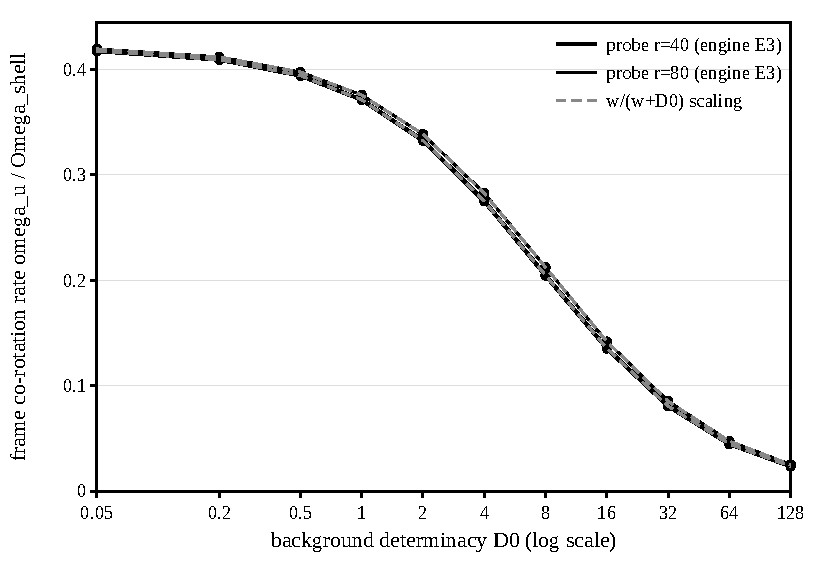
\includegraphics[width=\columnwidth]{fig1.pdf}
\caption{\label{fig:mach}%
局所慣性系の共回転率 $\omega_u/\Omega_{\rm shell}$ を内部プローブ点
($r = 40, 80$;各4方位)で測ったものと背景確定度 $\Dz$(対数スケール)
の関係。破線は重み分率スケーリング $\bar w/(\bar w+\Dz)$。
\texttt{tools/gen-figures.mjs} により,スクリプト内に明示されたバケツ
リング構成(固定リング源14個,$r = 150$,$m = 80$,
$\Omega_{\rm shell}=0.012$)で $\Dz \in \{0.05,\dots,128\}$ を走らせ,
エンジンのフレーム配列(規則 E3)を読んで生成;測定曲線とスケーリングは
$<0.1\%$ で一致する。}
\end{figure}

\subsection{実験2:増幅された引きずりによる外縁速度増強}
\label{sec:exp2}

円盤系を\emph{同一の}初期条件から $k_F = 1$ と $k_F = 0$(内蔵の
ニュートン対照,第\ref{sec:newton}節)で2回走らせる。構成は2つ:表示用
プリセット \texttt{galaxy}(中心 $m = 600$ +円盤粒子 $n = 380$,
$r \le 260$,$\Dz = 1$)と縮小検証構成 V11(同じ中心質量,$n = 140$,
$r \le 130$,$\Dz = 0.5$;\ref{app:inputs})である。
$k_F = 1$ では集団回転がフレーム場 $u_\varphi(r)$ に供給され,外縁の星は
回転するフレームに移流されて外縁の $v(r)$ が上がる;$k_F = 0$ の対照
曲線は,明示された動径区間でほぼケプラー的な減少を示す。
機械ゲート(検査 V11)は縮小構成の外縁帯($r \in [85,130]$)平均接線
速度差をステップ 1000--2000 で時間平均して測る:ゲイン $0.055$
(ゲート $\ge 0.03$),対照ドリフト $0.012$。表示用プリセットに対する
図生成ゲートは 6000 ステップ時点の外縁帯比
$v_{\varphi}(k_F{=}1)/v_{\varphi}(k_F{=}0) = 1.082$ を測る。
どちらの数値も単一シード構成によるものである;系統的な複数シードの
不確かさ研究は今後の課題とする。
この主張のゲートは意図的に速度\emph{増強}に置き,平坦性には置かない:
平均速度差は曲線の傾きを測らないし,この $N = 140$ 円盤について外縁の
対数傾き $\beta = \ud\ln v_\varphi/\ud\ln r$ を直接推定するとノイズ支配に
なる(外縁帯でのビン化最小二乗フィットは帯・ビン化・時期に依存して
$\beta \approx -0.2$ から $-0.5$,ケプラー的 $-0.5$ に対して;6000
ステップの単一時点スナップショットでは対照の $-0.47$ に対し
$\beta = -0.24$;表示用プリセットについての引用値)。
したがって誠実な機械ゲート付きの言明は,ケプラー的傾きより浅いか同程度の
傾きを伴う\emph{緩やかな外縁速度増強}であり,平坦区間の実証ではない。
自己無撞着なフレーム解析はさらに\emph{背景クロスオーバースケール}
$r_{\rm bg} \sim M_d/\Dz$ を与える。これを超えると背景確定度が円盤の
フレーム寄与を遮蔽し,いかなる増強も消えなければならない
($u_\varphi \to 0$,ケプラー的回復);$\Dz$ スキャンによる折れ半径の
測定は検証済みの予言としてではなく,任意の演習として残す。
本実験はモデル内部での機構のデモンストレーションである;否定的主張2を
参照。

\begin{figure}[t]
\centering
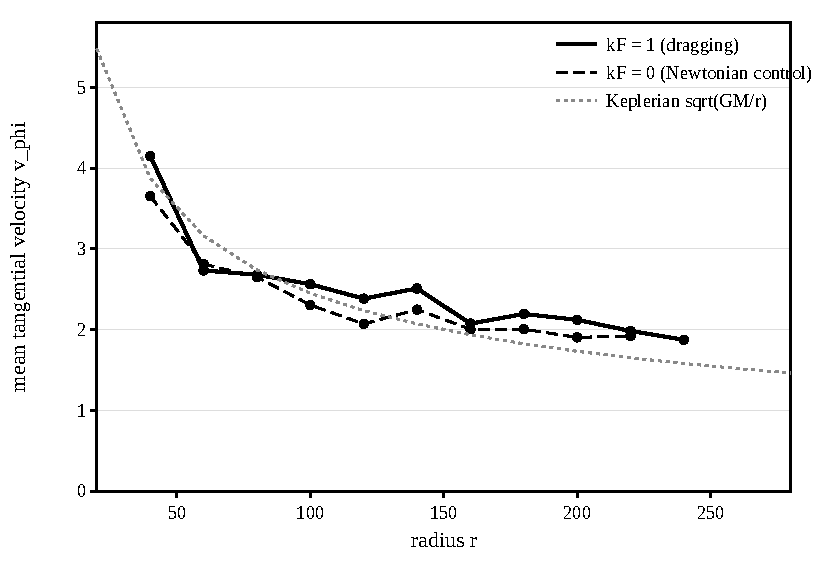
\includegraphics[width=\columnwidth]{fig2.pdf}
\caption{\label{fig:galaxy}%
同一初期条件に対する回転曲線 $v_\varphi(r)$:$k_F = 1$(外縁速度の
増強)と $k_F = 0$(ケプラー的対照),ケプラー期待値を重ねて表示。
表示用プリセット \texttt{galaxy}(中心 $m{=}600$,円盤 $n{=}380$,
$r{\le}260$,準ケプラー初期化 $\times1.05$,$\Dz{=}1$)の内蔵 A/B 比較
モードで生成(6000 ステップ時点の外縁帯比 $1.082$);別立ての縮小検証
構成 V11($n{=}140$,$r{\le}130$,$\Dz{=}0.5$)は時間平均外縁帯ゲインを
$0.055$(ゲート $\ge 0.03$)でゲートする。}
\end{figure}

\subsection{実験3:近点後退とその反転}
\label{sec:exp3}

固定されたスピンする中心の周りの離心試験軌道($a = 60$,$e = 0.5$)を,
$k_F \in \{0,1\}$ と中心スピン $S = \pm0.05$ で積分する。
自動検査 V6 は $-7.52^\circ$/周回(順行スピン:後退),
$+10.71^\circ$/周回(スピン反転:前進),$k_F = 0$ の数値対照で
$-1.03^\circ$/周回を測る---符号はスピン反転で反転し,ゲートは効果が
数値対照ドリフトの3倍を超えることを要求する(測定された順行効果は対照の
約7倍)。
別途規定した追加構成($a=120$,$e=0.5$,$S=+0.01$)は
$-2.445^\circ$/周回を与えて $S$ にほぼ線形にスケールし,連続極限公式
式~(\ref{eq:prec}) は符号・スピンスケーリング・大きさのオーダーを再現
する(遠方場核近似に対する測定係数 $c_p \approx 0.33$)。
長時間ロゼット構成(\texttt{tools/gen-figures.mjs} 内に明示;かつての
\texttt{drag} プリセットで,バージョン 1.24 で測地線プリセット
\texttt{mercury} に置き換えて廃止)は,軌道トレイルの描くロゼットとして
同じ物理を示す(その構成のパラメータで $-11.3^\circ$/周回,
図\ref{fig:drag}a)。

\begin{figure}[t]
\centering
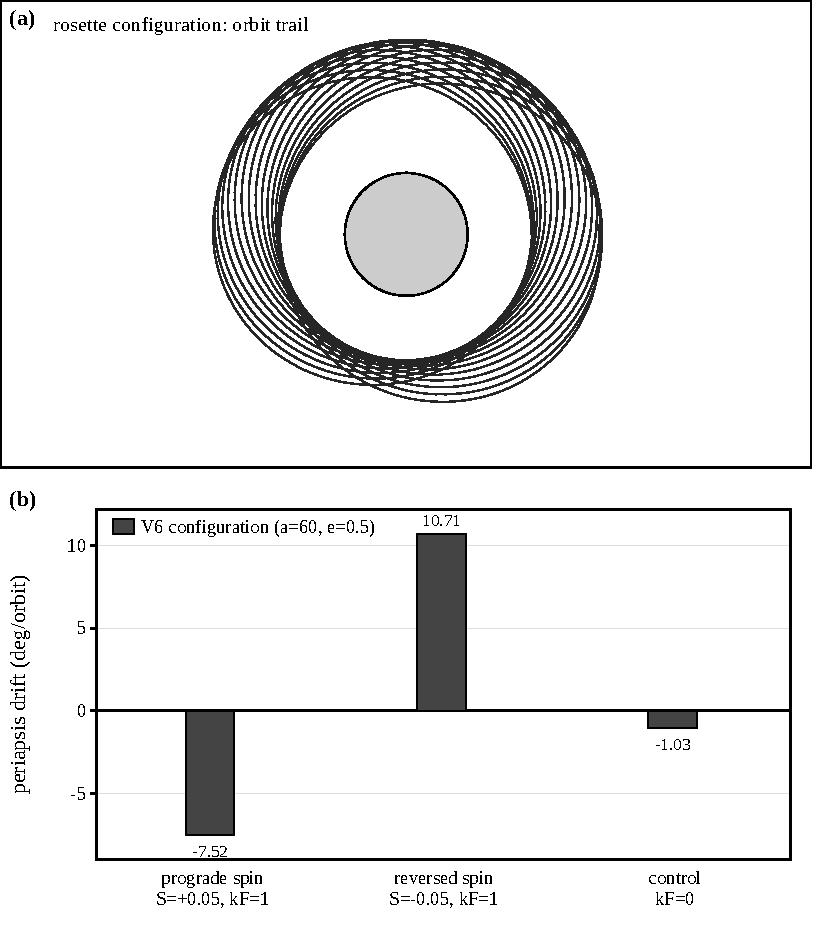
\includegraphics[width=\columnwidth]{fig3.pdf}
\caption{\label{fig:drag}%
(a)~ロゼット構成(中心 $m{=}600$,$S{=}0.09$,$(60,0)$ から
$v_y{=}3.87$ の試験軌道)での $\sim$8 周回の軌道トレイル:楕円は軌道
運動と逆向きに歳差し(後退),ロゼットを描く。
(b)~中心スピン符号に対する周回あたり近点ドリフト:順行スピンで後退
$-7.52^\circ$,反転スピンで前進 $+10.71^\circ$,$k_F{=}0$ の対照で
$-1.03^\circ$。
\texttt{tools/gen-figures.mjs} により V6 構成($a{=}60$,$e{=}0.5$,
$S{=}\pm0.05$,$k_F\in\{0,1\}$,$\Dz{=}0.05$,散逸オフ;$r$ ゲートと
最小間隔による近点検出)とロゼット構成(168\,000 ステップ)から生成。}
\end{figure}

\subsection{実験4:時計---重力+運動,そして双子}
\label{sec:exp4}

3つの機械検査が E7R を解析値に対して検査する:
(i) 純運動学的な遅れ(V12):重力項を抑制した状態で,
$v/c_0 = 0, 0.3, 0.6$ において $\tau/t = 1.0000/0.9540/0.8001$,理論値
$1/0.9539/0.8000$(最大相対誤差 $9.1\times10^{-5}$);
(ii) 円軌道上の重力+運動の複合的遅れ(V13):$\tau/t = 0.8629$,解析値
との相対誤差 $6.8\times10^{-6}$;この検査は自己場除外の検出器を兼ねる;
(iii) 双子構成(V16):局所フレームで静止した基準時計に対する
$v = 0.5c_0$ の周回時計,$\tau_B/t = 0.8174$,$\tau_A/t = 0.9672$,
いずれも解析積分に一致し,折り返しでどの時計にも不連続はない
(ステップ間変動 $4.8\times10^{-7}$)。
DFM の優先系表現では,双子の帰結は式~(\ref{eq:A7}) の平明な世界線積分で
ある;相対的同時性の「パラドックス」にまつわる概念装置は一切登場しない。
モデル文書に記録された限界の画定を強調する:これは\emph{表現}の簡略化で
あって相対論の反証ではない---標準的な相対論もまた,固有時積分によって
双子を一意に解決する。
重力項のみはプリセット \texttt{gclock} で対話的に表示される:中心質量
から距離を増しながら置いた3つの静止時計が $\tau/t = 0.931/0.965/0.979$
で時を刻み,解析値に一致する(以前のリリースの専用双子プリセットは
バージョン 1.24 で廃止;双子構成そのものは機械検査 V16 として残る)。

\begin{figure}[t]
\centering
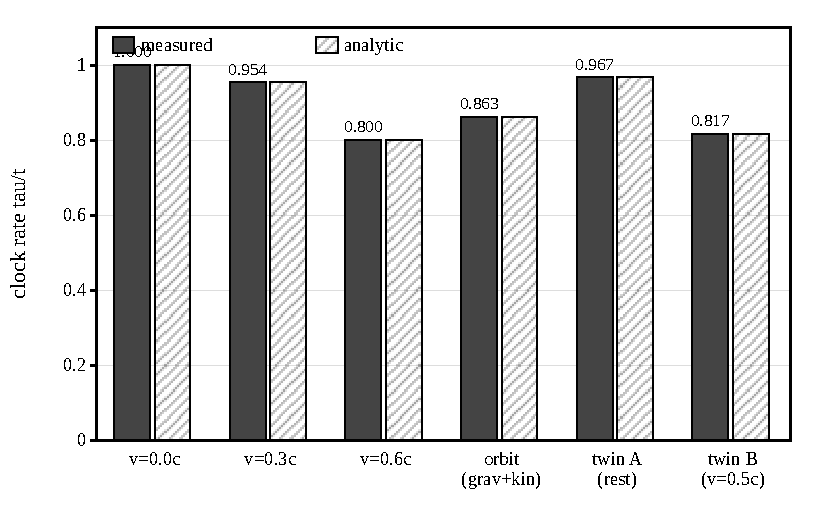
\includegraphics[width=\columnwidth]{fig4.pdf}
\caption{\label{fig:clocks}%
運動学的(V12),重力$+$運動複合(V13),双子(V16)構成における
時計レート $\tau/t$ の測定値と解析値;全6時計での最悪相対偏差は
$9.1\times10^{-5}$。
\texttt{tools/gen-figures.mjs} により V12/V13/V16 構成をそれぞれの
組み込みパラメータ(V12: $\Kt{=}10^6$,$v/c_0\in\{0,0.3,0.6\}$;
V16: $v{=}0.5c_0$)で各 1000 ステップ走らせて生成;重力項の対話的な
対応物:プリセット \texttt{gclock}。}
\end{figure}

\subsection{実験5:光---偏向,捕獲,非対称な屈曲}
\label{sec:exp5}

26本の平行光線ファンをコンパクトな質量の場に通す(プリセット
\texttt{lensing},$\Kt = 150$):平均屈曲角 $48.6^\circ$,うち5本は
積分の間持続する周回経路に捕獲される---光子球の光学的アナロジーである
(ブラックホールや事象の地平線の物理の主張は行わない)。
スピンする中心(プリセット \texttt{spinlens})では,光線ファンの両側が
不均等に曲がる---式~(\ref{eq:E8}) の媒質移流項 $\vect{u}$ が順行光線を
速め,逆行光線を遅らせる(カー的な光学非対称,T8)。
機械ゲート V8(係数感度のため $\Kt = 500$ で実行)は非対称度を
$6.77\times10^{-2}$~rad と測り,中心スピンに比例する。

\begin{figure}[t]
\centering
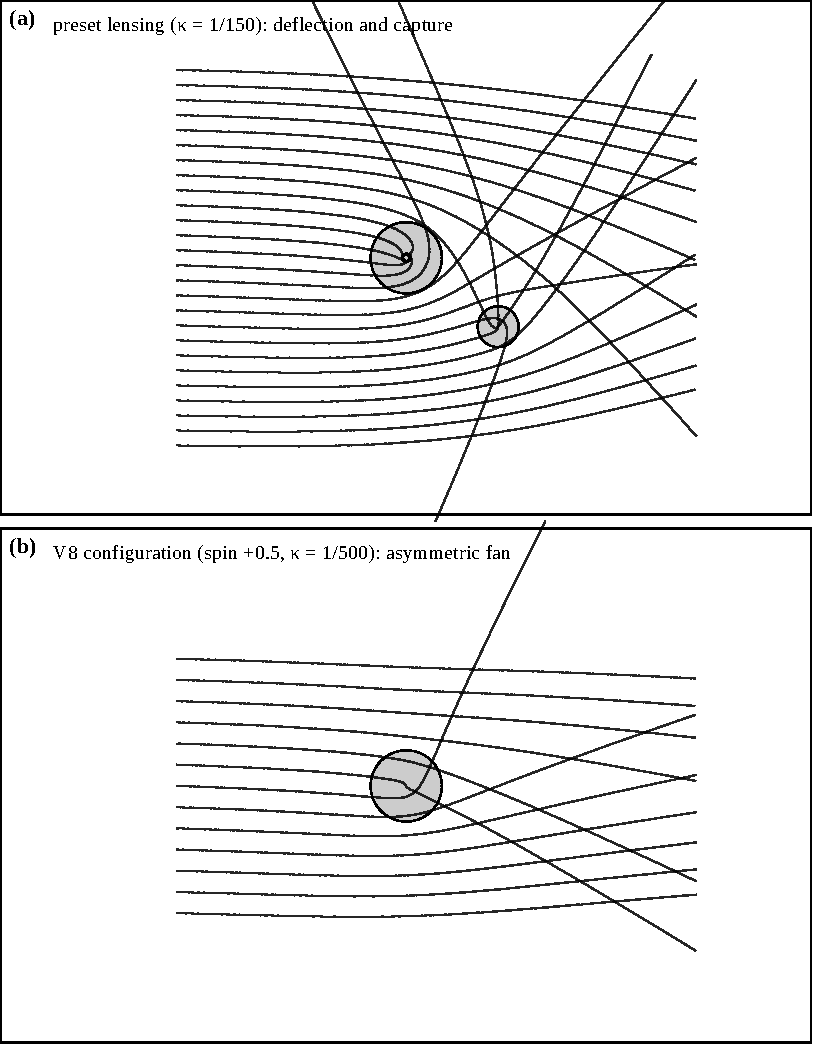
\includegraphics[width=\columnwidth]{fig5.pdf}
\caption{\label{fig:light}%
(a)~プリセット \texttt{lensing} の光線ファン($\Kt{=}150$,26本,
$x_0{=}-300$,$|y_0|\le255$,$\ud l{=}2.73$):質量への偏向と捕獲された
周回光線(光子球の光学的アナロジー)。
(b)~V8 構成の光線ファン(中心質量 1500,スピン $+0.5$,$\Kt{=}500$):
媒質が回転フレームに移流されるため,上半分と下半分が不均等に曲がる。
\texttt{tools/gen-figures.mjs} により共有光線トレーサ(規則 E8R)経由で
生成;定量ゲート:検証ルーチン V8,非対称度
$\pm6.77\times10^{-2}$~rad,スピン反転で符号反転。}
\end{figure}

\subsection{実験6:スピン=熱---平衡化と圧力}
\label{sec:exp6}

2つのデモを示す。いずれもスピンの一様性と温度の一様性が一致する単一
粒径に限定する(L9):
(i) 高温/低温に分けた気体(プリセット \texttt{gas};自己重力と
引きずりをオフにした統制構成)は,接触摩擦とスピン拡散を通じて左右の
平均温度を平衡化する---第0法則アナロジー T6;
(ii) 低温殻内の高温コア(プリセット \texttt{pressure})は膨張し,加熱
された粒子のスピン反発が殻を外へ押す(平均コア半径 $34.5 \to 140.9$,
軽い行き過ぎの後に落ち着く $4.1$ 倍の膨張)---課された
スピン依存ペア力 E5$'$ が巨視的な外向き応力を生む;課されて\emph{いない}
のは巨視的な圧力法則である。
\texttt{gas} ランは散逸的である(ギャップが閉じる間,記帳チャネルが系
全体を冷やす)ため,CI スイートの\emph{孤立対照}で平衡化と冷却を分離
する:冷却と接触のチャネルをすべてオフ
($\eta_{\rm rad} = \gamma_n = \mu_f = 0$;スピン拡散 E10$'$ のみ)に
した静的な高温/低温格子は,温度ギャップを単位時間あたり測定レート
$1.8\times10^{-3}$ で指数関数的に閉じ,その間,全スピン角運動量
$\sum_i I_i s_i$ は丸め床まで保存される。同じランの2体版は
式~(\ref{eq:E10}) の解析緩和レート $\kappa_s\,g(d)$ を相対誤差
$3\times10^{-5}$ で再現する。
したがって平衡化は拡散規則そのものの性質であり,すべてがゼロへ減衰する
ことの副産物ではない。
スペクトル温度計(検査 V2)は A9 と A12$'$ を結ぶ代数的往復検査を
与える:ウィーン逆変換 $s(\lambda) = \sqrt{b_m/(I\lambda)}$ が放射色の
生成に使われたスピンを $5\%$ 以内で回復する(記帳の整合性検査であって
独立測定ではない)。
否定的主張6の画定を繰り返す:これらは定性的アナロジーである;モデルの
状態方程式は理想気体の $\rho T$ ではなく $\rho^2 T$ でスケールし
(L15),定量的な熱力学的主張は行わない。
単一粒径制限の理由は,粒径が不揃いだと E10$'$ が温度 $T = I s^2$ では
なく角速度 $s$ を均すため,等分配が破れて,より冷たい小粒子からより
熱い大粒子へ熱が流れうるからである---だからこそ本稿の定量的な熱デモは
すべて単一粒径を用いる(L9)。

\begin{figure}[t]
\centering
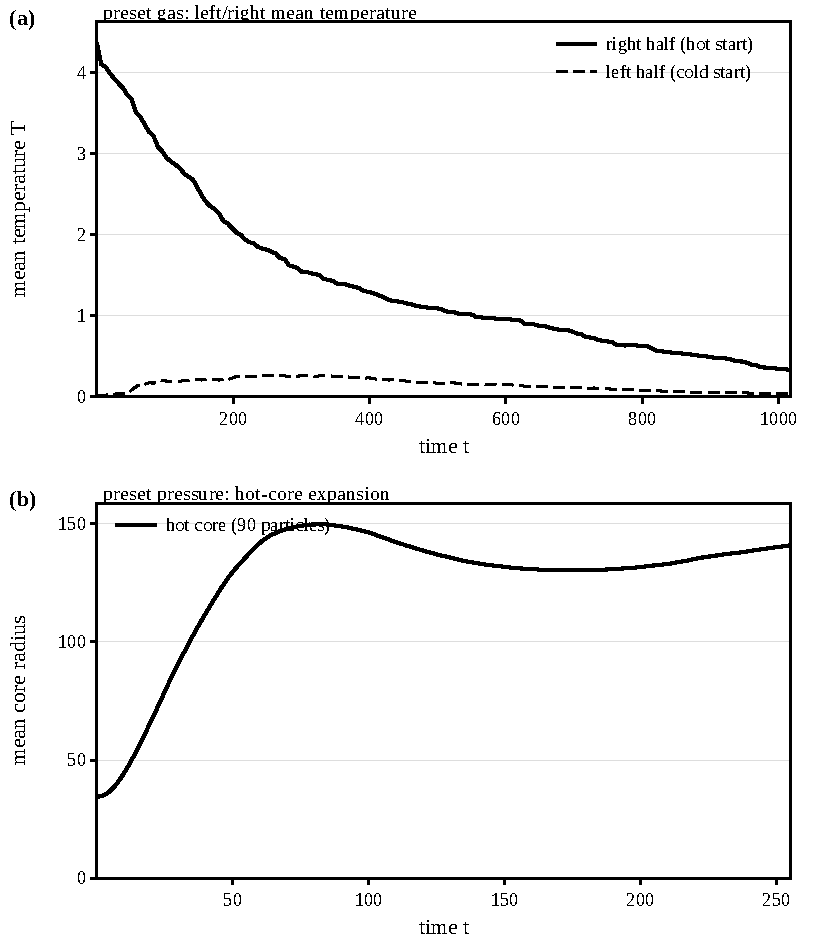
\includegraphics[width=\columnwidth]{fig6.pdf}
\caption{\label{fig:heat}%
(a)~プリセット \texttt{gas}(単一粒径)の左右平均温度時系列:初期
ギャップ $4.4$ が $0.29$ へ閉じる一方,全熱量は記帳された散逸チャネル
(A12$'$)を通じて減衰する---共通の,ゆっくり冷えていく温度への均一化。
(b)~プリセット \texttt{pressure} における低温殻に抗する高温コアの膨張:
平均コア半径 $34.5 \to 140.9$。
\texttt{tools/gen-figures.mjs} により名前付きプリセットを既定パラメータ
(それぞれ 64\,000 および 16\,000 ステップ)で \texttt{HP.sim} 経由で
実行して生成。}
\end{figure}

% =====================================================================
\section{限界と否定的主張}
\label{sec:negative}

以下の6つの言明は,論文に付け足された免責事項ではなく,論文の主張の
一部である。
L$n$ として参照される未解決問題は,プロジェクトの導出文書に目録化されて
いる(第\ref{sec:repro}節)。

\subsection{否定的主張1:実宇宙の記述ではない}
DFM は自然の記述として提案されるものではない。
これは\emph{計算的思考実験}である:反実仮想的な公理系---「もし空間が
純粋に関係論的で,引きずりが強かったら?」---の帰結の研究である。

\subsection{否定的主張2:ダークマターについて何も述べない}
外縁速度増強のデモ(実験2)は,ダークマターが不要であることを含意
しない。
実宇宙では GR のフレーム引きずりは $v/c^2$ で抑制されて桁違いに弱く,
ダークマターに関わる観測的証拠(CMB 非等方性,重力レンズ統計,構造
形成)は独立で強固である~\cite{Planck2018}。
実験2は\emph{モデル内部での}機構の十分性を示す。それ以上ではない。

\subsection{否定的主張3:ローレンツ不変性なし,因果的伝播なし}
フレーム $\vect{u}$ と場 $W$ は大域配置から瞬時に設定され(L8),物質は
ローレンツ的応答を持たない(L12):運動する装置に対する片道光速の
等方性は再現されない。
その帰結として,モデルは重力波放射による連星パルサーの軌道減衰を原理的に
記述できない。

\subsection{否定的主張4:2次元のみ}
モデルは2次元である;3次元の定量的予言は行わない。
スピンはスカラーである;3次元拡張(ベクトルスピン,ベクトル引きずり場,
角運動量整列)は今後の課題である(L7)。

\subsection{否定的主張5:基本力学は水星の近日点前進を再現しない}
観測される主要項($+42.98''$/世紀)は静的 1PN 効果である。
DFM の静的セクターは厳密にニュートン的であり(第\ref{sec:newton}節),
その引きずり項 E6$'$ は異なる動径冪を持つレンズ=ティリング符号の
\emph{後退}しか与えない[式~(\ref{eq:prec})];単一の $k_F$ で複数の
惑星を同時に合わせることはできない(水星への強制フィットは金星を
$1.38$ 倍,地球を $1.63$ 倍,火星を $2.00$ 倍で外す)。
一方,時計・光セクターは $\Kt = c^2/G$ で公式レベルのベンチマーク一致を
示す(表\ref{tab:calib})---モデルはどのセクターが機能しどれが機能
しないかについて明示的である。
この主張は基本力学 E1$'$--E11 にスコープされ,不変のまま残る。
明示的にラベル付けされた測地線オプション E12(第\ref{sec:e12}節)は,
同じ $\Kt = c^2/G$ で追加の自由係数なしに完全な前進
($\beta = \gamma = 1$,$+42.98''$/世紀)を回復する(検査 V18/V20,
時間レートのみの対照 V19 は $1/3$);強い場と重力波の現象はどちらの
モードでもモデルの外に残る(L8,L12)。

\subsection{否定的主張6:熱力学はアナロジーである}
熱セクターは「温度代理 $T = Is^2$ と非局所反発を与えられた,角運動量を
持つ2次元散逸粒子系」である。
理想気体の状態方程式は再現しない(スピン圧力は $\rho^2T$ でスケールし,
既定の $q = 2$ では2次元ビリアル積分が箱サイズとともに対数発散する;
L15)。潜熱も相変数も含まない(固体/液体/気体デモは形態的アナロジーで
あり,潜熱的相転移の主張は行わない)。レイリー=ベナール臨界性も確立
しない(臨界レイリー数のスケーリング則についての主張は行わない)。
詳細釣り合いを欠く(正準平衡に収束する分子動力学ではなく,散逸的な
粒状系である;L16,L17)。粒径をまたぐ等分配は破れる(E10$'$ は
$T = Is^2$ ではなく角速度を均すので,不揃いな粒径間で低温から高温への
熱流がありうる;L9)。
定性的に成り立つのは,そして単一粒径についてのみ成り立つのは,次で
ある:温度平衡化,創発的圧力,伝導的輸送。

\subsection{未解決問題}
\label{sec:limits}

本稿に最も関係する目録:
{\bf L1}(作用原理:部分的に解決---E7R 線素の静的弱場測地線は測地線
オプション E12 として実装・機械検証済み(第\ref{sec:e12}節)だが,
E6$'$ 自体は依然として更新規則であり,$\vect{u}\ne0$ の統一が最重要の
未解決問題として残る,第\ref{sec:conclusion}節参照);
{\bf L8}(瞬時遠隔作用);
{\bf L12}(物質のローレンツ的応答の欠如);
{\bf L14}(宇宙論的 $\Dz$ スケール問題:全物質を数えると
$\Dz \sim 10^{27}\,{\rm kg\,m^{-1}} \approx \Kt$ になるが,回転曲線は
$\sim10^{20}$ を要求する---どの物質を数えるかの特定を要する7桁の緊張。
L8 と結びつく);
{\bf L15--L17}(熱力学セクター:非理想な状態方程式とその $q$ 依存性;
長距離伝導核;第1法則の主張領域を限定するスピン反発ポテンシャルの
記帳)。

% =====================================================================
\section{結論と今後の課題}
\label{sec:conclusion}

DFM は,意図的に最小限で意図的に反実仮想的な公理系がどこまで到達できる
かを示す:1つのスカラー場と1つのスピン自由度が,慣性・重力・引きずり・
時間の遅れ・光の屈曲・熱力学的挙動を単一の動作する実装の中で模倣し,
保存則は方程式レベルで厳密に満たされ,主要な数値結果はすべて自動検査で
検証される。
その教育的価値はまさに,機能する弱場セクター(表\ref{tab:calib})と
明確に画定された不一致(第\ref{sec:negative}節)の対にある:学習者は
同じ道具の中で\emph{両方}を見ることができ,ニュートン的対照は1つの
パラメータを変えるだけで得られる。

今後の課題として3つの方向を挙げる:

\paragraph*{(i) 作用原理と測地線(v2.0 の核)。}
このプログラムの静的な第1段階は既に測地線オプション E12 として実装・
機械検証されている(第\ref{sec:e12}節):線素 式~(\ref{eq:line}) の
静的弱場測地線は PPN $\beta = \gamma = 1$ を与え,1PN 近日点前進を回復
する。
残るプログラムは,物質・時計・光を単一の作用
$S = -mc^2\!\int\!\ud\tau$ から完全に導出することである:場の方程式,
$\vect{u}\ne0$ の測地線(E6$'$ の統一),自己場除外は未定義のままで
ある;成功すれば $k_F$ は回転のみのパラメータになる。
この統一をモデルの唯一最重要の未解決問題と位置づける。
分岐基準は事前に固定する:現行の E4/E6$'$ 力学が測地線の低速極限として
現れるなら v1 は v2 と連続である;そうでなければ v1 は現象論的トイと
して凍結され,v2 は別のモデルである。

\paragraph*{(ii) $\Dz$ スケール問題。}
まず背景/摂動分解 $W = W_{\rm bg}(t) + \delta W$ を,次に有限伝播速度を
持つ因果的な場を解析し,L14 の7桁の緊張に取り組む。

\paragraph*{(iii) 定量熱力学プロファイル。}
状態方程式スキャンのための別パラメータプロファイル($q = 3$,有限
レンジ伝導,周期境界)を,天体物理的デモから切り離して整備する。

\section*{再現性と付随ツール}
\label{sec:repro}
\addcontentsline{toc}{section}{再現性と付随ツール}

完全なモデル---エンジン,22のプリセット,検証スイート,文書(公理,
導出,および全外部 AI 査読ラウンドの裁定記録)---は外部依存のない単一
HTML ファイルであり,プロジェクトリポジトリとともにアーカイブされて
いる。
コードは MIT ライセンス,文書は CC~BY~4.0 で
\url{https://github.com/tty-imamura/dfm-simulator} にて公開される。
本論文の記録版は注釈付きリポジトリタグ \texttt{paper-v1}(リリース
v1.27.0 系)で固定され,Zenodo に
\href{https://doi.org/10.5281/zenodo.21454189}%
{doi:10.5281/zenodo.21454189} としてアーカイブされている。これにより
論文中のすべての数値が1つの不変コミットに結びつく。
機械検証の出力もその記録の一部である:継続的インテグレーション
スイート(\texttt{tests/qa.mjs},組み込み \texttt{HP.verify.all()}
検査・表\ref{tab:verify}の時間刻みスイープ・第\ref{sec:exp6}節の孤立
第0法則対照を含む 109 項目)は機械可読な結果ファイル
(\texttt{tests/out/qa-results.json},git コミットを刻印)を書き出し,
後述の図ごとの JSON 記録とともに補足資料としてアーカイブされる;本稿で
引用した検証ランの正確な構成(全物理パラメータ,シード,ステップ数)は
\ref{app:inputs}に列挙する。
本稿のすべての図は,スクリプト \texttt{tools/gen-figures.mjs}
(リポジトリの一部)によってシミュレーションから再生成される。この
スクリプトは各キャプションに明示されたプリセットと検証ルーチンを実行し,
各図の隣に生成パラメータと測定値の JSON 記録を出力する。
付随ツールには弱場較正プリセット(\texttt{grcal})も含まれる。これは
表\ref{tab:calib}の数値をモデル内アナロジーと並べて表示する:地上時計と
周回衛星時計のレート($\tau/t = 0.920$ 対 $0.971$)が GPS オフセットの
符号構造---重力が運動に勝る---を再現し,付随する屈折を光線ファンが示す。

\section*{謝辞}
\addcontentsline{toc}{section}{謝辞}
数学的定式化,実装,検証は AI システム(Anthropic Claude)との協働で
行った;外部 AI 査読(ChatGPT,Grok,Gemini)を敵対的検査として用いた。
すべての公理と最終判断は著者によるものである。

% =====================================================================
\appendix

\section{SI 単位の復元}
\label{app:si}

シミュレータは $G = 1$ の無次元単位である。
理想($\varepsilon \to 0$)公式について:

\begin{table}[h]
\caption{\label{tab:si}弱場対応の SI 復元。}
\centering
\small
\setlength{\tabcolsep}{4pt}%
\begin{tabular}{lp{0.40\columnwidth}p{0.24\columnwidth}}
\toprule
量 & 値 & 備考 \\
\midrule
$[W]$ & ${\rm kg\,m^{-1}}$ & 確定度の次元 \\
$\Kt = c^2/G$ & $\approx 1.35\times10^{27}\ {\rm kg\,m^{-1}}$ &
時計/光の係数 \\
$2/\Kt = 2G/c^2$ & $\approx 1.48\times10^{-27}\ {\rm m\,kg^{-1}}$ &
実効レンズ係数 \\
\bottomrule
\end{tabular}
\end{table}

実効レンズ係数 $2/\Kt$ は導出された組合せであり
(第\ref{sec:dynamics}節,E8R),モデルの独立パラメータではない。
ソフトニング $\varepsilon$ は長さの次元を持つが数値的正則化にすぎない;
引用した物理的比較は $\varepsilon \to 0$ 極限を指す。

較正定数が\emph{線密度}(kg\,m$^{-1}$)であることの物理的直観:確定度
$W = \sum m/d$ 自体が質量/長さの次元を持ち,$\psi = W/\Kt$ が1の
オーダーに達するのはちょうど $GM/(c^2 d) \sim 1$,すなわち相対論的に
コンパクトな系の質量対半径比においてである。
同じ組合せは観測可能な宇宙の質量対半径スケール
($GM_u/(c^2R_H) \sim 1$,シアマの一致)としても,GR 文献で論じられる
「最大力」$c^4/4G = \tfrac14(c^2/G)\,c^2$ としても再帰する。

% =====================================================================
\section{ベンチマーク入力と検証ラン構成}
\label{app:inputs}

表\ref{tab:inputs}は表\ref{tab:calib}の弱場ベンチマーク行の背後にある
すべての入力を固定する;これらの値と $\Kt = c^2/G$ により,同表の各
数値はそれ以上の選択なしに再計算可能である。
全行に2つの規約を適用する:モデルの光速は $c_0 = c$,太陽系構成は
フレーム場に対して静止($\vect{u} = 0$;このとき式~(\ref{eq:A7}) の
DFM 速度は通常の軌道速度)とする。
固有時レートは常に時計自身の場を除外する($W_{\rm ext}$,A7$'$)。

\begin{table}[h]
\caption{\label{tab:inputs}%
ベンチマーク行(表\ref{tab:calib})の観測入力。
値は標準参照値である:基礎定数は CODATA~\cite{CODATA2022} と整合,
太陽・惑星量は IAU 2015 公称値~\cite{Prsa2016} と整合,GPS の軌道・
速度・時計オフセット入力は標準的な GPS 相対論文献~\cite{Ashby2003}
による。}
\centering
\small
\setlength{\tabcolsep}{4pt}%
\begin{tabular}{p{0.34\columnwidth}p{0.36\columnwidth}p{0.16\columnwidth}}
\toprule
入力 & 値 & 使用先 \\
\midrule
$M_\oplus$ & $5.972\times10^{24}$ kg & GPS \\
$R_\oplus$(地上時計) & $6.371\times10^{6}$ m & GPS \\
$r_{\rm GPS}$(軌道半径) & $2.6562\times10^{7}$ m & GPS \\
$v_{\rm sat} = \sqrt{GM_\oplus/r_{\rm GPS}}$ & $3.87$ km/s & GPS \\
$v_{\rm ground} = \Omega_\oplus R_\oplus$ & $0.465$ km/s & GPS \\
$M_\odot$ & $1.989\times10^{30}$ kg & 偏向,シャピロ \\
$R_\odot$($=b$) & $6.96\times10^{8}$ m & 偏向,シャピロ \\
$r_1$(地球) & $1\ {\rm AU} = 1.496\times10^{11}$ m & シャピロ \\
$r_2$(土星) & $8.43\ {\rm AU} = 1.261\times10^{12}$ m & シャピロ \\
幾何 & 外合,往復 & シャピロ \\
\bottomrule
\end{tabular}
\end{table}

表\ref{tab:vconfig}は本文で引用した検証ランの構成を固定する。
すべてのランは決定論的である:ランダムな天体は,明示されたプリセット
ID から導かれるシードを持つシード付き生成器から生成されるので,同一
ID は同一初期条件を再現する(CI 検査が強制する)。
記載のないパラメータはエンジン既定値を取る;積分器の刻みは V1 スイープ
を除き $\ud t = 0.016$ である。

\begin{table}[h]
\caption{\label{tab:vconfig}%
検証ラン構成(組み込みスイート;プリセット ID \texttt{verify\_v1} 等が
決定論的レイアウト生成器をシードする)。}
\centering
\small
\setlength{\tabcolsep}{4pt}%
\begin{tabular}{p{0.17\columnwidth}p{0.72\columnwidth}}
\toprule
ラン & 構成 \\
\midrule
V1 & $\Dz{=}0$,$k_F{=}1$,$G{=}1$,$k_{\rm rep}{=}1$,
$\mu_f{=}0.5$,$\gamma_n{=}0.4$,$\kappa_s{=}0.05$,
$\eta_{\rm rad}{=}0$,$\varepsilon{=}2$;中心 $m{=}30$($s{=}0.5$)
$+$ 円盤 $n{=}48$,$r{\le}120$,$m\in[0.5,2]$,$s\in[-2,2]$,
ランダム速度($\times1.2$);1000 ステップ
(スイープ:$T{=}16$ 固定で $\ud t \in \{0.016,0.008,0.004\}$) \\
V9 & $G{=}1$,$\Dz{=}2$,$\varepsilon{=}2$;原点に固定 $m{=}50$,
$(18,-7)$ に $m{=}20$,3点にプローブ $m{=}0.01$;中心差分
$h{=}0.01$ \\
V10 & $G{=}1$,$\Dz{=}0$,$k_F{=}0$,$k_{\rm rep}{=}0$,
$\mu_f{=}0.5$,$\gamma_n{=}0.4$,$\kappa_s{=}0.3$,
$\eta_{\rm rad}{=}2\times10^{-4}$($p{=}1$),$\varepsilon{=}2$;
37粒子(中心 $m{=}30$,$s{=}0.8$ $+$ 円盤 $n{=}36$,$r{\le}55$,
$m\in[1,2]$,$s\in[-1.5,1.5]$);1000 ステップ \\
V10b & $G{=}0$,$k_{\rm rep}{=}2$,全散逸オフ;明示位置の3粒子
$m{=}2,3,2.5$,スピン $2,-1.5,1$;1000 ステップ \\
V11 & $G{=}1$,$\Dz{=}0.5$,$\mu_f{=}0.02$,$\gamma_n{=}0.05$,
$k_{\rm rep}{=}1$,$\kappa_s{=}0.05$,$\varepsilon{=}4$;中心
$m{=}600$($s{=}0.05$)$+$ 円盤 $n{=}140$,$r{\le}130$,
$m\in[0.5,1.2]$,準ケプラー($\times1.05$);同一初期条件から
$k_F{=}1/0$ の A/B;外縁帯 $r\in[85,130]$,ステップ 1000--2000 で
時間平均 \\
第0法則対照 & $G{=}0$,$k_F{=}0$,$k_{\rm rep}{=}0$,
$\mu_f{=}\gamma_n{=}\eta_{\rm rad}{=}0$,$\kappa_s{=}0.3$;
$8\times6$ 静的格子(間隔 40),$m{=}1$,スピン $0.3$(左)/
$2.5$(右),4000 ステップ;2体版 $m{=}2$,$d{=}30$,スピン
$2/0$,2500 ステップ \\
V18--V20 & $G{=}1$,$\Dz{=}0.05$,$k_F{=}0$,$k_{\rm rep}{=}0$,
全散逸オフ,$\Kt{=}10^4$,$c_0{=}40$,\texttt{geoPN}{=}1,
$\varepsilon{=}0.5$;原点に固定源 $m{=}150$,$(47.664,0)$ に試験
粒子 $m{=}0.01$,$v_y{=}1.94787$($a{=}60$,$e{=}0.2056$);
3ラン $(\alpha,\lambda_{\rm PN}) = (1.5,1)/(0.5,1)/(1.5,0)$,
各 80\,000 ステップ;$r$ ゲートと最小間隔による近点検出 \\
\bottomrule
\end{tabular}
\end{table}

% =====================================================================
\section{帰結 T1--T9}
\label{app:theorems}

表\ref{tab:theorems}は本文で参照した帰結を,依存関係・成立条件・
(存在する場合)機械ゲートとともに列挙する。
特定の初期条件とパラメータ範囲についてのみ妥当性が確立された項目は
\emph{条件付き数値命題}(CNP)と記す;これらは定理ではない。

\begin{table*}[t]
\caption{\label{tab:theorems}%
帰結 T1--T9:言明,依存関係,ステータス,機械ゲート。
CNP $=$ 条件付き数値命題(検証済み構成で成立;一般性は主張しない)。}
\centering
\small
\begin{tabular}{lp{0.34\textwidth}p{0.13\textwidth}p{0.14\textwidth}p{0.19\textwidth}}
\toprule
ID & 言明 & 依存 & ステータス & 機械ゲート \\
\midrule
T1 & $N{=}1$,$\Dz{=}0$ のとき:粒子自身の位置で(自己を含む)
フレームは $\vect{v}_1$ に等しく,E6$'$/E7R の自己除外フレームは
未定義($W_{\rm ext}{=}0$)---単一粒子の運動を検出しうる基準は
存在しない & A3, A4 & 構成的言明 & (構成的;V12 のフレーム処理に
入る) \\
T2 & 支配的質量の近傍で $\vect{u} \to \vect{v}_j$:空間は引きずられ
る;$\Dz \gg \sum w$ では $\vect{u} \to 0$ & A3, A4 & 極限言明 &
実験1のスケーリング $\bar w/(\bar w{+}\Dz)$,$<0.1\%$ \\
T3 & 接触摩擦は軌道を円化しスピンを整列させる(2次元) &
A9, E9 & CNP & プリセットデモ(\texttt{saturn}) \\
T4 & 集団的円盤回転は $u_\varphi$ に供給される;外縁軌道速度は
$k_F{=}0$ 対照より増強される(外縁速度増強;平坦性主張なし) &
A5, E3, E6$'$ & CNP & V11(ゲイン 0.055,ゲート $\ge$0.03);
表示プリセット比 1.082 \\
T5 & 光は $n_{\rm eff} = e^{2\psi}$ で質量へ向かって曲がる;強い場は
光線を捕獲する(光子球の光学的アナロジー) & A7$'$, A11, E8R &
弱場公式 $+$ CNP & 偏向公式(表\ref{tab:calib});プリセット
\texttt{lensing} での捕獲 \\
T6 & スピン=熱は温度を平衡化し(第0法則アナロジー),圧力を生む
(単一粒径でのみ有効) & A9, A10, E5$'$, E9, E10$'$ &
CNP(単一粒径;L9) & \texttt{gas} / \texttt{pressure} ゲート;
孤立第0法則対照(第\ref{sec:exp6}節) \\
T7 & $\Dz{=}0$,固定粒子なしのとき:$\vect{P}$ と $L_{\rm tot}$ は
厳密に保存;$\Dz{>}0$ の欠損はリザーバ台帳に等しい & A13, E4,
E5$'$, E6$'$, E9, E10$'$ & 方程式レベルの定理
(証明は第\ref{sec:dynamics}節) & V1(残差は丸め床,
$\ud t$ 非依存) \\
T8 & スピンする中心は順行光線と逆行光線を不均等に曲げる。非対称度
$\propto k_F u_\varphi$(カー的光学アナロジー) & A8, A11, E8R &
CNP & V8(非対称度 $6.77\times10^{-2}$ rad,スピンで符号反転) \\
T9 & 再会時の時計差は式~(\ref{eq:A7}) の一意な世界線積分である;
「相互の時間の遅れ」は観測者中心の同期がもたらす表現効果である
(相対論の反証ではない---表現の簡略化) & A11, E7R & 表現に関する
言明 & V16(双子時計は解析積分に一致;不連続なし) \\
\bottomrule
\end{tabular}
\end{table*}

% =====================================================================
% 参考文献(英語版と同一。全項目は一次/準一次記録に対して 2026-07-18 に
% 検証済み;独立 AI 査読3系統でクロスチェック)
\begin{thebibliography}{99}

\bibitem{Newton1687}
I.~Newton, \emph{Philosophi\ae{} Naturalis Principia Mathematica}
(Jussu Societatis Regi\ae{} ac Typis Josephi Streater, Londini, 1687),
Scholium to the Definitions.

\bibitem{Mach1883}
E.~Mach, \emph{Die Mechanik in ihrer Entwickelung:
historisch-kritisch dargestellt} (F.~A.~Brockhaus, Leipzig, 1883);
English trans.\ T.~J.~McCormack, \emph{The Science of Mechanics:
A Critical and Historical Exposition of Its Principles}
(Open Court Publishing Co., Chicago, 1893).

\bibitem{Sciama1953}
D.~W.~Sciama, ``On the origin of inertia,''
Mon.\ Not.\ R.\ Astron.\ Soc.\ \textbf{113}, 34--42 (1953),
\href{https://doi.org/10.1093/mnras/113.1.34}
{doi:10.1093/mnras/113.1.34}.

\bibitem{BarbourBertotti1982}
J.~B.~Barbour and B.~Bertotti, ``Mach's principle and the structure of
dynamical theories,''
Proc.\ R.\ Soc.\ Lond.\ A \textbf{382}, 295--306 (1982),
\href{https://doi.org/10.1098/rspa.1982.0102}
{doi:10.1098/rspa.1982.0102}.

\bibitem{LenseThirring1918}
J.~Lense and H.~Thirring, ``\"Uber den Einflu\ss{} der Eigenrotation
der Zentralk\"orper auf die Bewegung der Planeten und Monde nach der
Einsteinschen Gravitationstheorie,''
Phys.\ Z.\ \textbf{19}, 156--163 (1918),
ADS bibcode: 1918PhyZ...19..156L; English translation in
Gen.\ Relativ.\ Gravit.\ \textbf{16}, 727--741 (1984),
\href{https://doi.org/10.1007/BF00759853}{doi:10.1007/BF00759853}.

\bibitem{Everitt2011}
C.~W.~F.~Everitt \emph{et al.}, ``Gravity Probe B: Final results of a
space experiment to test general relativity,''
Phys.\ Rev.\ Lett.\ \textbf{106}, 221101 (2011),
\href{https://doi.org/10.1103/PhysRevLett.106.221101}
{doi:10.1103/PhysRevLett.106.221101}.

\bibitem{CiufoliniPavlis2004}
I.~Ciufolini and E.~C.~Pavlis, ``A confirmation of the general
relativistic prediction of the Lense--Thirring effect,''
Nature \textbf{431}, 958--960 (2004),
\href{https://doi.org/10.1038/nature03007}{doi:10.1038/nature03007}.

\bibitem{RubinFord1970}
V.~C.~Rubin and W.~K.~Ford, Jr., ``Rotation of the Andromeda nebula
from a spectroscopic survey of emission regions,''
Astrophys.\ J.\ \textbf{159}, 379--403 (1970),
\href{https://doi.org/10.1086/150317}{doi:10.1086/150317}.

\bibitem{Milgrom1983}
M.~Milgrom, ``A modification of the Newtonian dynamics as a possible
alternative to the hidden mass hypothesis,''
Astrophys.\ J.\ \textbf{270}, 365--370 (1983),
\href{https://doi.org/10.1086/161130}{doi:10.1086/161130}.

\bibitem{Planck2018}
Planck Collaboration, ``Planck 2018 results. VI. Cosmological
parameters,'' Astron.\ Astrophys.\ \textbf{641}, A6 (2020),
\href{https://doi.org/10.1051/0004-6361/201833910}
{doi:10.1051/0004-6361/201833910};
Erratum: Astron.\ Astrophys.\ \textbf{652}, C4 (2021),
\href{https://doi.org/10.1051/0004-6361/201833910e}
{doi:10.1051/0004-6361/201833910e}.

\bibitem{CooperstockTieu2005}
F.~I.~Cooperstock and S.~Tieu, ``General relativity resolves galactic
rotation without exotic dark matter,'' arXiv:astro-ph/0507619 (2005),
\href{https://arxiv.org/abs/astro-ph/0507619}
{arXiv:astro-ph/0507619}.

\bibitem{FuchsPhleps2006}
B.~Fuchs and S.~Phleps, ``Comment on `General relativity resolves
galactic rotation without exotic dark matter','' New Astron.\
\textbf{11}, 608--610 (2006),
\href{https://doi.org/10.1016/j.newast.2006.04.002}
{doi:10.1016/j.newast.2006.04.002}.

\bibitem{Korzynski2007}
M.~Korzy\'nski, ``Singular disk of matter in the Cooperstock--Tieu
galaxy model,'' J.\ Phys.\ A: Math.\ Theor.\ \textbf{40}, 7087--7092
(2007),
\href{https://doi.org/10.1088/1751-8113/40/25/S66}
{doi:10.1088/1751-8113/40/25/S66}.

\bibitem{Ludwig2021}
G.~O.~Ludwig, ``Galactic rotation curve and dark matter according to
gravitomagnetism,'' Eur.\ Phys.\ J.\ C \textbf{81}, 186 (2021),
\href{https://doi.org/10.1140/epjc/s10052-021-08967-3}
{doi:10.1140/epjc/s10052-021-08967-3}.

\bibitem{LasenbyHobsonBarker2023}
A.~Lasenby, M.~P.~Hobson, and W.~Barker, ``Gravitomagnetism and galaxy
rotation curves: a cautionary tale,'' Class.\ Quantum Grav.\
\textbf{40}, 215014 (2023),
\href{https://doi.org/10.1088/1361-6382/acef8b}
{doi:10.1088/1361-6382/acef8b}.

\bibitem{deFelice1971}
F.~de~Felice, ``On the gravitational field acting as an optical
medium,'' Gen.\ Relativ.\ Gravit.\ \textbf{2}, 347--357 (1971),
\href{https://doi.org/10.1007/BF00758153}{doi:10.1007/BF00758153}.

\bibitem{Unruh1981}
W.~G.~Unruh, ``Experimental black-hole evaporation?''
Phys.\ Rev.\ Lett.\ \textbf{46}, 1351--1353 (1981),
\href{https://doi.org/10.1103/PhysRevLett.46.1351}
{doi:10.1103/PhysRevLett.46.1351}.

\bibitem{BarceloLiberatiVisser2005}
C.~Barcel\'o, S.~Liberati, and M.~Visser, ``Analogue gravity,''
Living Rev.\ Relativity \textbf{8}, 12 (2005),
\href{https://doi.org/10.12942/lrr-2005-12}{doi:10.12942/lrr-2005-12}.

\bibitem{LyndenBellKatz1995}
D.~Lynden-Bell and J.~Katz, ``Classical mechanics without absolute
space,'' Phys.\ Rev.\ D \textbf{52}, 7322--7324 (1995),
\href{https://doi.org/10.1103/PhysRevD.52.7322}
{doi:10.1103/PhysRevD.52.7322}.

\bibitem{Assis1999}
A.~K.~T.~Assis, \emph{Relational Mechanics}
(Apeiron, Montreal, 1999).

\bibitem{Bertotti2003}
B.~Bertotti, L.~Iess, and P.~Tortora, ``A test of general relativity
using radio links with the Cassini spacecraft,''
Nature \textbf{425}, 374--376 (2003),
\href{https://doi.org/10.1038/nature01997}{doi:10.1038/nature01997}.

\bibitem{Verlinde2017}
E.~Verlinde, ``Emergent gravity and the dark universe,''
SciPost Phys.\ \textbf{2}, 016 (2017),
\href{https://doi.org/10.21468/SciPostPhys.2.3.016}
{doi:10.21468/SciPostPhys.2.3.016}.

\bibitem{BrilliantovPoschel2004}
N.~V.~Brilliantov and T.~P\"oschel,
\emph{Kinetic Theory of Granular Gases}
(Oxford University Press, Oxford, 2004),
\href{https://doi.org/10.1093/acprof:oso/9780198530381.001.0001}
{doi:10.1093/acprof:oso/\allowbreak 9780198530381.001.0001}.

\bibitem{IorioMercury2011}
L.~Iorio, ``Mercury and frame-dragging in light of the MESSENGER
flybys: towards a new test of general relativity?''
arXiv:1109.0266 (2011),
\href{https://arxiv.org/abs/1109.0266}{arXiv:1109.0266}.

\bibitem{IorioEtAl2011}
L.~Iorio, H.~I.~M.~Lichtenegger, M.~L.~Ruggiero, and C.~Corda,
``Phenomenology of the Lense--Thirring effect in the Solar System,''
Astrophys.\ Space Sci.\ \textbf{331}, 351--395 (2011),
\href{https://doi.org/10.1007/s10509-010-0489-5}
{doi:10.1007/s10509-010-0489-5}.

\bibitem{Ashby2003}
N.~Ashby, ``Relativity in the Global Positioning System,''
Living Rev.\ Relativity \textbf{6}, 1 (2003),
\href{https://doi.org/10.12942/lrr-2003-1}{doi:10.12942/lrr-2003-1}.

\bibitem{CODATA2022}
P.~J.~Mohr, D.~B.~Newell, B.~N.~Taylor, and E.~Tiesinga,
``CODATA recommended values of the fundamental physical constants:
2022,'' Rev.\ Mod.\ Phys.\ \textbf{97}, 025002 (2025),
\href{https://doi.org/10.1103/RevModPhys.97.025002}
{doi:10.1103/RevModPhys.97.025002}.

\bibitem{Prsa2016}
A.~Pr\v{s}a \emph{et al.}, ``Nominal values for selected solar and
planetary quantities: IAU 2015 Resolution B3,''
Astron.\ J.\ \textbf{152}, 41 (2016),
\href{https://doi.org/10.3847/0004-6256/152/2/41}
{doi:10.3847/0004-6256/152/2/41}.

\end{thebibliography}

\end{document}
